\chapter{Understanding Surrogate Model Accuracy in Bayesian Optimisation}
\label{ch:ch08:noisy_oracle}

\section{Introduction}

Bayesian optimisation (\gls{bo}) has emerged as a powerful technique for solving black-box optimisation problems, particularly for functions that are expensive to evaluate. The ability of \gls{bo} to efficiently reach good solutions within relatively few evaluations has made it an important approach in a variety of domains, ranging from hyperparameter tuning in machine learning~\citep{SnoEtAl12} to engineering design~\citep{JonEtAl98} and scientific discovery~\citep{LooEtAl19}. Bayesian optimisation relies on a surrogate model, which serves as a (computationally) inexpensive approximation of the objective function. This surrogate model is used to predict both the value of the objective function at unobserved points and the uncertainty associated with those predictions. These predictions are then combined by means of an acquisition function, which balances the trade-off between exploring unknown regions of the search space and exploiting regions known to contain high-quality solutions~\citep{Garnett23}.

The surrogate model is a key component of Bayesian optimisation algorithms. Among the most commonly used surrogate models are Gaussian processes (GPs), which 
can be seen as a probabilistic model of a given objective function~\citep{RasWil06}. 
While GPs offer many advantages, notably flexibility and the ability to quantify uncertainty, they also have limitations; for instance, their computational cost scales poorly with the number of observations.

Furthermore, due to their continuous nature, GPs cannot model categorical inputs naturally. Beyond GPs, other models, including random forests \citep{HutEtAl11}, deep neural networks \citep{BalajiLakshminarayanan17} and conformal predictors \citep{ShaVov08}, have been employed as surrogates, each with their own strengths and weaknesses. The choice of surrogate model can significantly influence the performance of a Bayesian optimisation procedure, and therefore, it is of considerable interest to understand how these models perform under different conditions.

One of the key challenges in evaluating surrogate models is determining how their accuracy impacts the overall optimisation process. In traditional machine learning tasks, model performance is often assessed using metrics such as accuracy, mean squared error or log-likelihood on a held-out test set. However, these metrics may not directly correlate with optimisation performance in the context of Bayesian optimisation. For example, while it is commonly assumed that higher accuracy near the optimum is more important than accuracy in other regions (see, e.g., \citealp{Frazier18}), 
inaccuracies in less critical regions can still have detrimental effects. Such inaccuracies may lead to misleading acquisition function values, ultimately causing the optimiser to waste evaluations in suboptimal areas of the search space.  \changed{However, to the best of our knowledge, no prior work validated these assumptions and conducted a through evaluation.}

\changed{In this work, we aim to understand what makes the prediction of a surrogate model effective for Bayesian optimisation. }
\changed{Towards this end, we introduce the \textit{noisy oracle} surrogate model,}
which provides noisy predictions of the ground-truth values of the objective function. The level of noise is determined by a weighting scheme that reflects the importance of different regions of the search space. By systematically varying these weighting schemes, we can study how accuracy in different regions influences the optimisation process itself, rather than a simple aggregation of prediction error. With this methodology we aim to achieve a targeted view of surrogate-model quality.
Using it in a series of computational experiments, we find evidence that a good surrogate model needs to be accurate in regions where the target function has good values, and that being accurate only around the optimum can still result in suboptimal \gls{bo} performance.

\changed{We support our empirical experiments with a theoretical analysis that derives explicit conditions under which each acquisition function (EI, PI, LCB) is guaranteed to prefer a suboptimal point over the optimum due to a mistake in the peredictions of the surrogate model. These conditions depend on the noise assigned to the suboptimal point, the objective gap, and the predictive uncertainty, providing a formal basis for the empirical observation that value-based schedules are more robust than distance-based ones.

We note that, while real surrogate models might suffer from problems such as oversmoothing~\citep{HvaEtAl24}, uncalibrated uncertainty predictions~\citep{FolEtAl23}, heteroskedastic noise~\citep{CowEtAl22} and other types of error, our goal here is to take a first step towards understanding a more general question: where in the optimisation landscape does the surrogate model need to be accurate to effectively support Bayesian optimisation, independent of the details of a particular surrogate class. By simplifying the surrogate to an oracle with controlled noise, we aim to isolate the accuracy question from other factors such as uncertainty calibration, model class, and learning dynamics. We view this as a necessary foundation upon which future work can build by progressively relaxing these simplifications.

In the following sections, we first review existing approaches to surrogate-model evaluation and related assumptions regarding surrogate model accuracy. We then formalise the noisy oracle framework and introduce the weighting schemes used in our experiments. Next, we present an empirical evaluation of how these different accuracy patterns affect optimisation performance, followed by an analysis of how a GP and a random forest behave on a real optimisation trajectory. We then provide theoretical analysis of the noisy oracle framework. Finally, we conclude with implications for the design of Bayesian optimisation algorithms and surrogate models.}

\section{Background}
Given a black-box function $f:\sR^n\rightarrow\sR$, the goal of an optimiser is to find its minimum, denoted by $x^*$, such that $f(x^*)\leq f(x)$ for every $x\in\sR^n$. The optimiser iteratively samples configurations $x_1, x_2, ..., x_n$, where $x_i$ is the configuration sampled at iteration $i$.
At each iteration, the optimiser observes the performance $f(x_i)$, producing the set of observations $\train=\{(x_1, f(x_1)), (x_2, f(x_2)),..., (x_n, f(x_n))\}$.

Bayesian optimisation~\citep{Garnett23} uses a surrogate model to decide on the next configuration to sample. At iteration $i$, the surrogate model $S$ takes an unseen configuration $x$ together with the observation set $\train$ and estimates a predictive distribution for $x$, typically summarized through a mean $\mu_S(x)$ and variance $\sigma_S^2(x)$.
GPs are a common choice for such a surrogate model, but random forests~\citep{HutEtAl11} and other machine-learning techniques that can provide uncertainty estimates are also used.

Following the fitting of a surrogate model, an acquisition function is used to determine the next point to sample, balancing exploration and exploitation by considering the predicted mean and variance. Here, we consider three popular acquisition functions. First, expected improvement (EI) quantifies the expected improvement in the known optimum by sampling a configuration $x$; formally:
\begin{multline}
    EI(x)=\mathbb{E}[max(0, f(x_{best})-\mu_S(x))]=\\(f(x_{best})-\mu_S(x))\cdot\Phi(z)+\sigma_S(x)\cdot\phi(z)
\end{multline}

\begin{equation*}
    z=\frac{f(x_{best})-\mu_S(x)}{\sigma_S(x)},
\end{equation*}
where $f(x_{best})=\min_{j=1, 2, ..., n} f(x _j)$ is the best observed function value up to iteration $n$, also known as the incumbent.
Similarly, probability improvement (PI) quantifies the probability that configuration $x$ improves over the known optimum:
\begin{equation*}
    PI(x)=P(f(x_{best})-\mu_S(x) > 0)=\Phi(z)
\end{equation*}
Finally, the lower confidence bound (LCB) is the weighted sum of the predicted performance $\mu_S(x)$ and the uncertainty $\sigma(x)$:
\begin{equation*}
    LCB(x)=-(\mu_S(x)-\lambda\sigma_S(x))
\end{equation*}

The acquisition function $AF$ is then optimised to find a candidate configuration $x_{next} \in \argmax_{x\in\sR^n}AF(x)$. Different methods have been proposed to optimise the acquisition function, including local search, evolutionary algorithms and gradient-based methods. Since evaluating the acquisition function is relatively cheap, many such evaluations can be used to obtain a strong candidate. The candidate is then evaluated on the target function $f$, after which $\train$ is updated as $\train=\train \cup \{(x_{next}, f(x_{next}))\}$. This process continues until a pre-defined evaluation budget is exhausted.

\section{Related Work}
In this section, we cover existing work related to our goal of assessing where surrogate models need to be accurate. We first look at local Bayesian optimisation approaches and then discuss several metrics for surrogate models.

\subsection{Local Bayesian optimisation}
Traditionally, Bayesian optimisation performed a global search over the entire search space. However, when the search space is large and high-dimensional, global search can be expensive. Local Bayesian optimisation methods have been introduced to solve this problem~\citep{EriEtAl19,NguEtAl22,PapEtAl22}. 
These methods focus on identifying candidates that are close to the current best 
solution. Most notably, TuRBO~\citep{EriEtAl19} uses \textit{trust regions} to limit the search space to a small region around the known best solutions. It then changes the size of the trust region based on the performance of the new solutions sampled. 

The success of such methods is due to their focus on the local region around the current best solution, which is often where the most promising candidates are found. By exploiting the structure of the objective function in this way, local Bayesian optimisation methods can achieve significant speedups over traditional global search strategies. This shows the assumption in the community that the surrogate model needs to be more accurate around the optimum.
A potential downside of local Bayesian optimisation methods is that they may continue exploring around a local optima, potentially missing better solutions elsewhere.
\changed{The success of local-Bayesian optimisation suggest that a surrogate model should have accurate predictions only around the optimum, an assumption we will check in the following sections.}

\subsection{Surrogate model evaluation}
Several metrics have been proposed to evaluate the quality of surrogate models. These include traditional regression metrics as well as metrics that are more specific to optimisation. In the following subsections, we review representative examples and highlight why they do not directly answer our question about where surrogate models need to be accurate for \gls{bo}.

\subsubsection{Mean squared error}
Mean squared error (MSE) is one of the most widely used regression metrics~\citep{EimEtAl25,GijEtAl24}; it summarises the squares of the errors for all samples in the test set. 
Formally, MSE is defined as:
\begin{equation*}
    MSE(f, \test)=\sum_{j=1}^{|\test|}(\mu_S(x_j)-f(x_j))^2
\end{equation*}
MSE can also be weighted by assigning different weights to individual points. Such weighting is performed in machine learning when dealing with unbalanced datasets or in cases where the domain expert determines that specific samples are more important. However, for Bayesian optimisation, there is no known weighting mechanism, and therefore all points are treated equally (for example in~\citet{SanEtAl23}).
    
\subsubsection{Ranking score}
Proposed by~\citet{FeuEtAl18} to create a weighted ensemble of pre-trained GPs, the ranking loss is based on the observation that the exact values of the configurations are less important in the optimisation context. Instead, we are interested in the best point, and therefore, the rank of the points is more important. The ranking loss is defined as:
\begin{equation*}
    \begin{aligned}
        RS(f, \test) = \sum_{j=1}^{|\test|} \sum_{k=1}^{|\test|} 
        \mathds{1} \Big\{ (f(x_j) < f(x_k)) \oplus \\
        \quad (\mu_S(y_j) < \mu_S(y_k)) \Big\}
    \end{aligned}
\end{equation*}
where $\oplus$ is the exclusive-or operation.

However, the ranking loss also treats all configurations equally. While we are interested in preserving the ranking of the points around the optimum, their rank far from the optimum has less impact. For example, given two configurations that are far from the optimum, we are only interested in knowing that they are far from it. The exact rank between these points is not important in the optimisation context. However, an error in ranking between these points will be taken into account in the same way as incorrect ranking between two points close to the optimum.


\subsubsection{Uncertainty evaluation} 
While in this work we put an emphasis on predicting the values obtained from the surrogate model, previous work has already researched the uncertainty of the model, as well as its expected calibration~\cite{FolEtAl23,KulEtAl18}, which is defined as:

\begin{equation*}
    ECE=\sum_{j=1}^{|\test|} (C_y(p)-p)^2
\end{equation*}
\begin{equation*}
    C_y(p)=\frac{1}{|\test|}\cdot \sum_{i\in \test} \mathbb{I}[y_i \leq F^{-1}_p(x_i)],
\end{equation*}

where $F^{-1}_p$ 
is the quantile function; this means that in a well-calibrated surrogate model, $p\%$  of the time, the test samples fall within $p\%$ of the confidence intervals, for several pre-defined $p$ values. The closer the ECE to $0$, the more calibrated the model is.

While other metrics to quantify surrogate models exist, such as log-likelihood and $R^2$ score, they all treat all samples equally, similarly to the other metrics we covered in this section.






\section{The noisy oracle surrogate model}
\begin{figure}
    \centering
    \hfill
    \begin{subfigure}[c]{0.30\textwidth}
        \centering 
        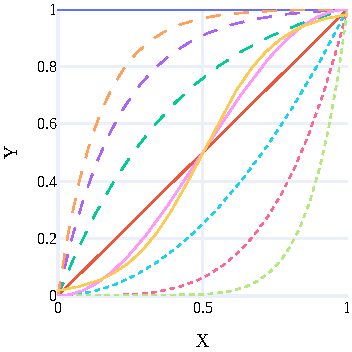
\includegraphics[width=0.8\textwidth]{figures/08/figures/schedule_functions_scaled.pdf}
        \caption{}
    \end{subfigure}
    \hfill
    \begin{subfigure}[c]{0.30\textwidth}
        \centering 
        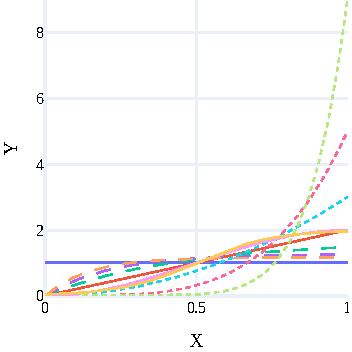
\includegraphics[width=0.8\textwidth]{figures/08/figures/schedule_functions_scaled_integral.pdf}
        \caption{}
    \end{subfigure}
    \hfill
    \begin{subfigure}[c]{0.38\textwidth}
        \centering

        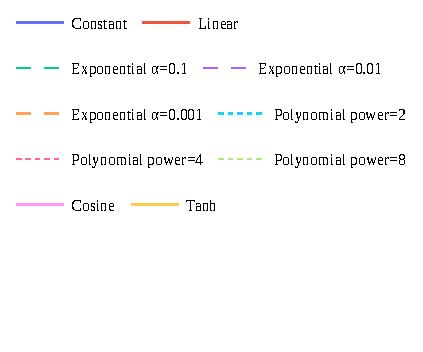
\includegraphics[width=1.0\textwidth]{figures/08/figures/schedule_functions_scaled_integral_legend_square.pdf}


    \end{subfigure}
    \hfill
    \caption[Original noise functions and schedules]{(a) Original noise functions. Note that different noise functions have different areas under the curve; hence, we normalise the different functions by dividing by their integral. (b) Normalised noise functions with equal area under the curve.}
    \label{fig:ch08:sched_funcs}
\end{figure}
We construct a noisy oracle surrogate model to assess where surrogate models need to be accurate. The noisy oracle is parameterised by a noise function $s:\sR\rightarrow\sR$ and a base noise level $N_\text{base}$. Like other surrogate models in Bayesian optimisation, the noisy oracle produces a predictive mean and variance for each candidate. The predictive mean returned for a candidate solution $x$ is
\begin{equation}
    \label{eq:ch08:noisy_mu1}
    \mu(x)=f(x)+\varepsilon_\mu(x)
\end{equation}
\begin{equation}
    \label{eq:ch08:noisy_mu2}
    \varepsilon_\mu(x)\sim\mathcal{N}(0, N(x))
\end{equation}
In other words, we add normally distributed noise $\varepsilon_\mu$ to the actual target function value $f(x)$. The value of $N(x)$ determines how noisy the returned sample value can be. A high $N(x)$ can cause a value 
$\mu(x)$ far from the actual function value, hence simulating a less accurate model for that solution. 



We define the uncertainty of the model as the general uncertainty
\begin{equation}
    \sigma(x)=N_{\text{base}}
\end{equation}

\changed{While real surrogate models typically induce more complicated uncertainty patterns, we keep the predictive uncertainty as the general noise level because our goal is to isolate the effect of the mean prediction. Varying $\sigma(x)$ simultaneously with the noise schedule would complicate the analysis, making it difficult to attribute performance differences to spatial accuracy patterns alone. Our theoretical results (Section~8) confirm that even with a varying $\sigma$, the misleading conditions still depend on $\sigma$ through the derived thresholds, showing that uncertainty plays a role but that the core phenomenon, distorted means misleading the acquisition function, is already present under constant uncertainty. We acknowledge that this simplification removes the data-driven exploration mechanism central to practical \gls{bo}. Our conclusions should therefore be interpreted as statements about where mean-prediction accuracy matters, holding uncertainty fixed. We note that studying the interaction between spatially varying $\sigma$ and mean-error patterns is an important direction for future work.}












The value of $N(x)$ can be determined from different measurements, such as how close $x$ is to the optimum $x^*$ or the value of $f(x)$. We denote by $m(x)$ the metric according to which the noise function is constructed, where lower values of $m(x)$ correspond to more important regions. Because different metrics can have different scales, we normalise $m(x)$ to the range $[0,1]$ using max-min normalisation:
\begin{equation*}
    \hat{m}(x)=\frac{m(x)-\min_{x'}{m(x')}}{\max_{x'}{m(x')}-\min_{x'}{m(x')}}
\end{equation*}
We then define the actual noise level $N(x)$ using the normalised metric $\hat{m}(x)$ together with a schedule $\hat{N}$ that expects an input in $[0,1]$:
\begin{equation*}
    N(x)=\frac{\hat{N}(x)(\hat{m}(x))}{\int_0^1\hat{N}(l)dl} \cdot N_\text{base} + N_\text{min}
\end{equation*}

Here, $N_\text{base}$ is the main noise level and $N_\text{min}$ is the minimum noise floor (set to $0.001$ in all experiments), ensuring that all solutions retain some prediction error. We further divide by the integral of the schedule so that all schedules have the same total area under the curve. This normalisation is important because some schedules would otherwise induce much less total noise than others and would therefore enjoy an unintended advantage unrelated to their shape.



\changed{We emphasise that the noisy oracle serves as the surrogate model in our \gls{bo} loop. When the acquisition function optimiser queries $\mu(x)$ at candidate points, it calls the noisy oracle and not the objective function directly. This is analogous to standard \gls{bo}, where acquisition optimisation queries the GP posterior (which itself was constructed from observed data). The objective $f(x)$ is used internally by the oracle to construct its prediction, but these internal accesses are not counted against the evaluation budget. Only the point ultimately selected by the acquisition function is evaluated on $f$ and added to the observation set $\mathcal{D}$. Each time $\mu(x)$ is queried, the noise term $\varepsilon_\mu(x)$ is sampled independently from $\mathcal{N}(0,N(x))$. This means that repeated queries to the same candidate $x$ within a single iteration may receive slightly different predictions, reflecting genuine stochastic variation in the surrogate rather than a deterministic lookup.}

\changed{Furthermore we note that, by design, the noisy oracle does not condition on the accumulated observations $\mathcal{D}$. We decided to do this to check what would be the performance of a specific model, without re-training. A data-dependent surrogate would complicate the effect of spatial accuracy patterns with the effect of learning dynamics, making it difficult to attribute performance differences to the noise schedule alone. Our noisy oracle can be viewed as examining a fixed snapshot of surrogate quality at each iteration.}

In the following, we study several noise functions $\hat{N}(x):[0,1]\rightarrow[0,1]$ to create a wide variety of functions, ranging from functions that give preference to only a small area around the optimum to more aggressive functions that allow wider areas to have less noise, at the expense of significantly higher noise for the rest of the landscape. The noise functions we consider are:
\begin{itemize}
    \item Linear
    \begin{equation*}
        \text{lin}(k)=k
    \end{equation*}
    \item Exponential with $v\in\{0.1, 0.001, 0.0001\}$
    \begin{equation*}
        \text{exp}_v(k)=\frac{1-v^k}{1-v}
    \end{equation*}
    \item Polynomial with $v\in\{2,4,8\}$
    \begin{equation*}
        \text{poly}_v(k)=k^v
    \end{equation*}
    \item Cosine
    \begin{equation*}
        \text{c}(k)=\frac{\cos{(\pi + k \cdot \pi)} +1}{2}
    \end{equation*}
    \item TanH
    \begin{equation*}
        \text{t}(x)=\frac{\tanh{(8 \cdot k - 4)} + 1}{2}
    \end{equation*}
    \item Constant
    \begin{equation*}
        \text{constant}(k)=1
    \end{equation*}
\end{itemize}

An illustration of the different noise functions is shown in \cref{fig:ch08:sched_funcs}, where we plot the functions before and after normalisation. The figure demonstrates that we included a wide variety of noise functions, ranging from those that yield low noise only for a minimal subset of solutions (e.g., Exponential with 0.01) to more relaxed noise functions that allow for larger areas to have lower noise levels. 

We study two ways of constructing the metric $m(x)$. First, we use the distance from the optimum, in which case solutions closer to the optimum receive more accurate predictions. Second, we use the target-function value itself, so that solutions with values closer to the optimum receive less noise even if they are not spatially close to $x^*$. Under this value-based construction, local optima with relatively good objective values can also receive accurate predictions.
These two constructions let us separate two competing notions of importance in \gls{bo}: geometric proximity to the optimum versus objective quality. 



\section{Experimental Evaluation}
\changed{
We present the results of our experiments with the noisy oracle in several stages. We begin by exploring value-based noise functions across different noise levels. We then turn to distance-based noise functions and compare their behaviour to the value-based variants. Next, we directly contrast the two noise types within each schedule family. We conclude the experimental section with checks over acquisition functions, acquisition function optimisers, and dimensionalities. Throughout, we report results on both the synthetic BBOB suite and the real-world PD1 benchmark.

\subsection{Setup of Experiments}
We experiment with both synthetic and real-world functions.
As synthetic functions, we used the BBOB~\citep{HanEtAl21} set through IOHExperimenter~\citep{DoeEtAl18}. BBOB contains 24 functions, ranging from a simple sphere function to more complex functions with various properties, such as multiple local optima or weak global structure. Each BBOB function has different instances, which are created by modifying the original function through rotation, the addition of constants and other transformations. 
We used the first 11 instances of each function and ran the optimisation using 5 pseudo-random seeds. We used dimensions 2, 4 and 8 of the BBOB functions.


We also used the PD1 surrogate-based benchmark~\citep{MalEtAl23}, which is a hyperparameter optimisation benchmark for neural networks. 
In PD1, each target function is a combination of a dataset and a neural network architecture (for example, wide ResNet on CIFAR100).
PD1 contains four target functions, and the goal is to optimise the hyperparameters of a neural network in order to minimise the error. PD1 contains purely continuous hyperparameters. We used 55 pseudo-random seeds in our PD1 experiments.

To compute the noise levels, we needed to know the location of the minimum and maximum of the target functions. For BBOB, the location of the minimum is already known from analytical solutions. To find the location of the maximal values, as well as the minimum and maximum of PD1, we ran 100 times three optimisation algorithms: differential evolution, L-BFGS-B~\citep{ByrEtAl95} and CMA-ES~\citep{HanOst01}, using default settings for all three algorithms. For the first two algorithms, we used  SciPy~\citep{VirEtAl19} implementation; for CMA-ES, we used the PyCMA~\citep{HanEtAl19} package. 
We chose these algorithms as they are popular optimisation procedures designed for non-constrained budgets (as opposed to Bayesian optimisation).

We implemented the noisy oracle surrogate model within the highly flexible SMAC3~\citep{LinEtAl22} Bayesian optimisation framework. We start each optimisation with one random sample, and then start the Bayesian optimisation loop using the noisy oracle, until we reach 100 samples. 

We performed our experiments on a compute cluster with 19 nodes; each node is equipped with two AMD EPYC 7543 32-Core processors with 512MB of L3 cache and 1TB of RAM running Rocky Linux 9.



\subsection{Value-based noise functions}

\begin{figure}
    \centering
    \begin{subfigure}{0.24\textwidth}
        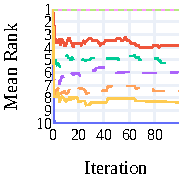
\includegraphics[]{figures/08/figures/noise_types_levels/rs_BBOBValueBased_2_0.01_ei_rank.pdf}
        \caption{0.01}
    \end{subfigure}
    \begin{subfigure}{0.24\textwidth}
        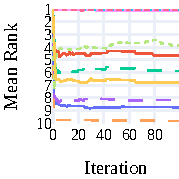
\includegraphics[]{figures/08/figures/noise_types_levels/rs_BBOBValueBased_2_0.05_ei_rank.pdf}
        \caption{0.05}
    \end{subfigure}
    \begin{subfigure}{0.24\textwidth}
        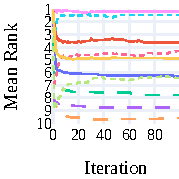
\includegraphics[]{figures/08/figures/noise_types_levels/rs_BBOBValueBased_2_0.1_ei_rank.pdf}
        \caption{0.1}
    \end{subfigure}
    \begin{subfigure}{0.24\textwidth}
        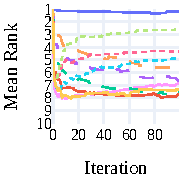
\includegraphics[]{figures/08/figures/noise_types_levels/rs_BBOBValueBased_2_0.2_ei_rank.pdf}
        \caption{0.2}
    \end{subfigure}
    \begin{subfigure}{0.24\textwidth}
        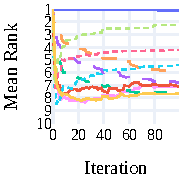
\includegraphics[]{figures/08/figures/noise_types_levels/rs_BBOBValueBased_2_0.3_ei_rank.pdf}
        \caption{0.3}
    \end{subfigure}

    \begin{subfigure}{0.24\textwidth}
        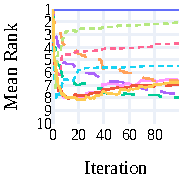
\includegraphics[]{figures/08/figures/noise_types_levels/rs_BBOBValueBased_2_0.5_ei_rank.pdf}
        \caption{0.5}
    \end{subfigure}

    \begin{subfigure}{\textwidth}
        \centering
        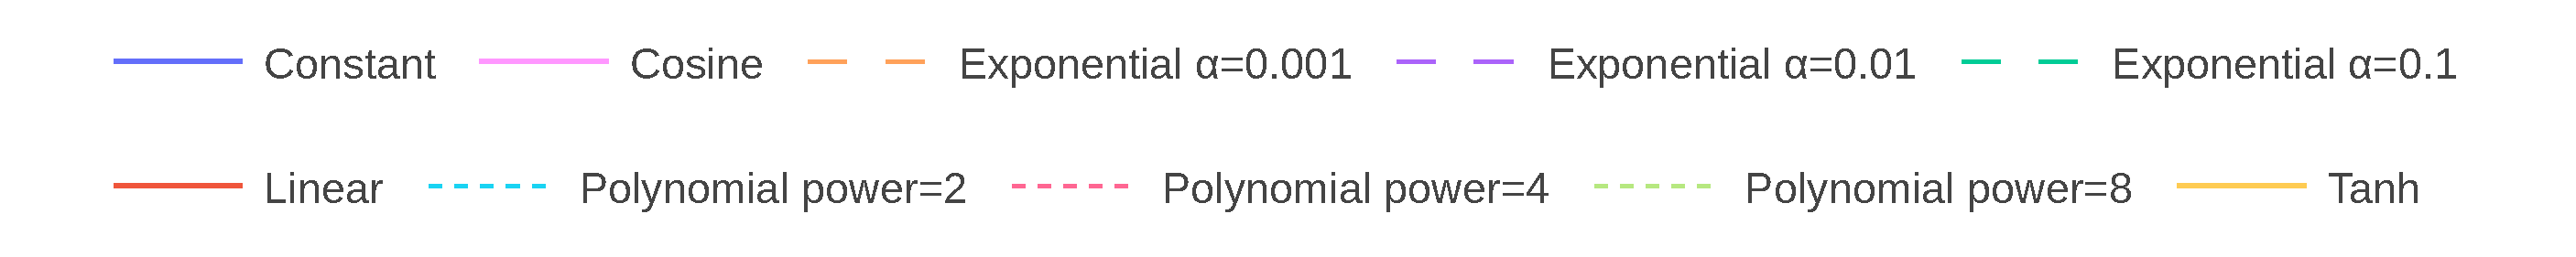
\includegraphics[scale=0.33]{figures/08/figures/noise_types_levels/rs_BBOBValueBased_2_0.3_ei_rank_legend.pdf}
    \end{subfigure}
    \caption[Value-based noise ranks on BBOB]{Mean ranks of regret resulting from running Bayesian optimisation with different value-based noise functions over different noise levels on the BBOB functions. For noise levels up to $0.1$, noise functions that give an advantage to larger areas around the optimum, at the expense of being more inaccurate far from it perform best. For higher noise levels, constant noise performs better.}
    \label{fig:ch08:value_based}
\end{figure}


We begin by examining the performance of the value-based noise functions.
\cref{fig:ch08:value_based} shows aggregated results over all 24 BBOB functions on dimension 2 with the EI acquisition function. Each sub-figure compares the different noise schedules at a given base-noise level. First, we observe that the ranking of the noise functions changes with the base noise level.

For low noise ($0.01$ and $0.05$), non-constant schedules that preserve larger low-noise regions around good objective values, such as the polynomial and cosine schedules, tend to achieve better final ranks than constant noise and than noise functions that leave very small areas with low noise (such as the exponential schedules).

At a noise level of $0.1$, the cosine schedule works best, followed by linear, polynomial with power of 4 and tanh. Constant noise performs better than polynomial with power of 8, which is the most aggressive polynomial schedule that assigns a major noise advantage to the largest proportion of solutions. This suggests that while allocating more accuracy to good-value regions is beneficial, the schedule should not be so aggressive that it assigns extreme noise to solutions that are only moderately suboptimal. Such solutions can still be competitive candidates for the acquisition function, and distorting their predictions too heavily can mislead the optimiser.

As the noise level increases ($0.2$--$0.5$), constant noise becomes the best noise function. Interestingly, however, the aggressive polynomial with power of 8 is more competitive at these high noise levels. A likely explanation is that at high base noise, all schedules produce substantial total distortion. Poly-8 concentrates nearly all of its noise budget on the worst-performing regions, effectively acting almost as a step function: points with very poor objective values receive extremely high noise, but this additional noise is unlikely to change their ranking since they are already clearly uncompetitive. Meanwhile, poly-8 assigns minimal noise to the top-performing fraction of the landscape. When the base noise level is already high, this extreme focus on protecting the best regions can be more beneficial than spreading the noise budget more evenly, because more moderate schedules may still leave even good regions with noticeable distortion.

\begin{figure}
    \centering
    \begin{subfigure}{0.24\textwidth}
        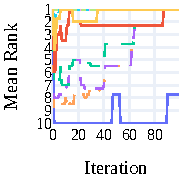
\includegraphics[]{figures/08/figures/noise_types_levels/rs_BBOBValueBased_0.01_ei_rank_pd1.pdf}
        \caption{0.01}
    \end{subfigure}
    \begin{subfigure}{0.24\textwidth}
        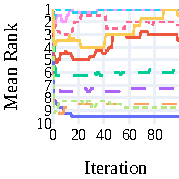
\includegraphics[]{figures/08/figures/noise_types_levels/rs_BBOBValueBased_0.05_ei_rank_pd1.pdf}
        \caption{0.05}
    \end{subfigure}
    \begin{subfigure}{0.24\textwidth}
        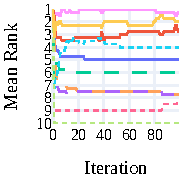
\includegraphics[]{figures/08/figures/noise_types_levels/rs_BBOBValueBased_0.1_ei_rank_pd1.pdf}
        \caption{0.1}
    \end{subfigure}
    \begin{subfigure}{0.24\textwidth}
        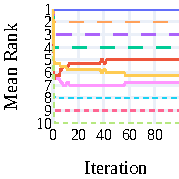
\includegraphics[]{figures/08/figures/noise_types_levels/rs_BBOBValueBased_0.2_ei_rank_pd1.pdf}
        \caption{0.2}
    \end{subfigure}
    \begin{subfigure}{0.24\textwidth}
        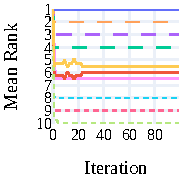
\includegraphics[]{figures/08/figures/noise_types_levels/rs_BBOBValueBased_0.3_ei_rank_pd1.pdf}
        \caption{0.3}
    \end{subfigure}
    \begin{subfigure}{0.24\textwidth}
        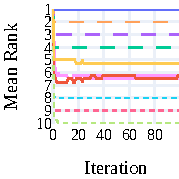
\includegraphics[]{figures/08/figures/noise_types_levels/rs_BBOBValueBased_0.5_ei_rank_pd1.pdf}
        \caption{0.5}
    \end{subfigure}
    \begin{subfigure}{\textwidth}
        \centering
        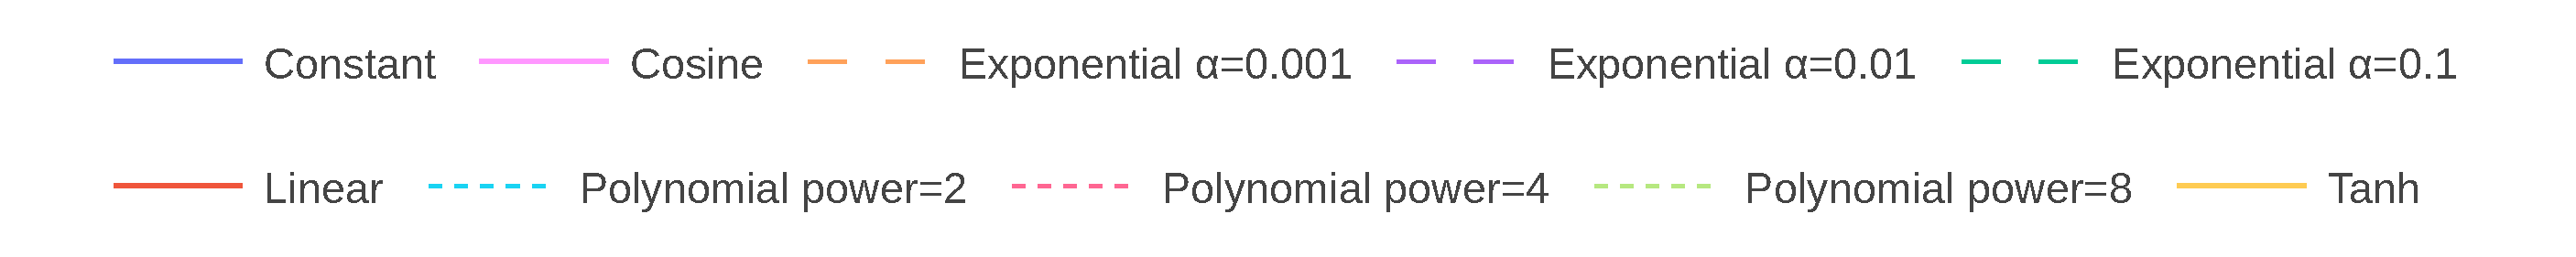
\includegraphics[scale=0.33]{figures/08/figures/noise_types_levels/rs_BBOBValueBased_0.3_ei_rank_pd1_legend.pdf}
    \end{subfigure}
    \caption[Value-based noise ranks on PD1]{Mean ranks of regret resulting from running Bayesian optimisation with different value-based noise functions over different noise levels on the real-world PD1 benchmark. Similar to the synthetic benchmark results, polynomial noise functions perform well at lower noise levels, whereas constant noise struggles significantly.}
    \label{fig:ch08:value_based_pd1}
\end{figure}


The PD1 results in \cref{fig:ch08:value_based_pd1} show a similar transition. At low-to-moderate noise levels, non-constant value-based schedules dominate: the cosine and tanh schedules perform very well, whereas overly aggressive or uniform schedules fare worse. The regime shift from non-constant to constant noise occurs at roughly the same noise level as on BBOB, despite the fact that PD1 contains only four target functions (compared to 24 for BBOB), suggesting that the transition is not an artefact of aggregation over many benchmarks. For higher noise levels, the less aggressive exponential schedules outperform the more aggressive non-constant schedules, while constant noise dominates overall.


\subsection{Distance-based noise}
\begin{figure}
    \centering
    \begin{subfigure}{0.24\textwidth}
        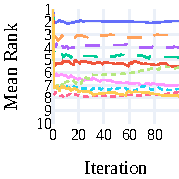
\includegraphics[]{figures/08/figures/noise_types_levels/rs_BBOBDistanceToOptimum_2_0.01_ei_rank.pdf}
        \caption{$N_\text{base}=0.01$}
    \end{subfigure}
    \begin{subfigure}{0.24\textwidth}
        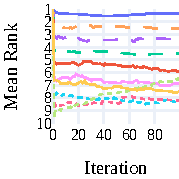
\includegraphics[]{figures/08/figures/noise_types_levels/rs_BBOBDistanceToOptimum_2_0.05_ei_rank.pdf}
        \caption{$N_\text{base}=0.05$}
    \end{subfigure}
    \begin{subfigure}{0.24\textwidth}
        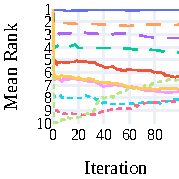
\includegraphics[]{figures/08/figures/noise_types_levels/rs_BBOBDistanceToOptimum_2_0.1_ei_rank.pdf}
        \caption{$N_\text{base}=0.1$}
    \end{subfigure}
    \begin{subfigure}{0.24\textwidth}
        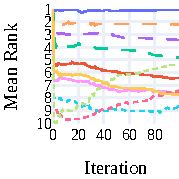
\includegraphics[]{figures/08/figures/noise_types_levels/rs_BBOBDistanceToOptimum_2_0.2_ei_rank.pdf}
        \caption{$N_\text{base}=0.2$}
    \end{subfigure}
    \begin{subfigure}{0.24\textwidth}
        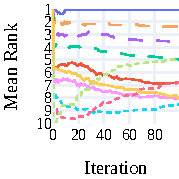
\includegraphics[]{figures/08/figures/noise_types_levels/rs_BBOBDistanceToOptimum_2_0.3_ei_rank.pdf}
        \caption{$N_\text{base}=0.3$}
    \end{subfigure}
    \begin{subfigure}{0.24\textwidth}
        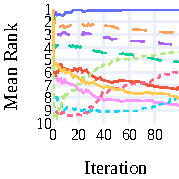
\includegraphics[]{figures/08/figures/noise_types_levels/rs_BBOBDistanceToOptimum_2_0.5_ei_rank.pdf}
        \caption{$N_\text{base}=0.5$}
    \end{subfigure}

    \begin{subfigure}{\textwidth}
        \centering
        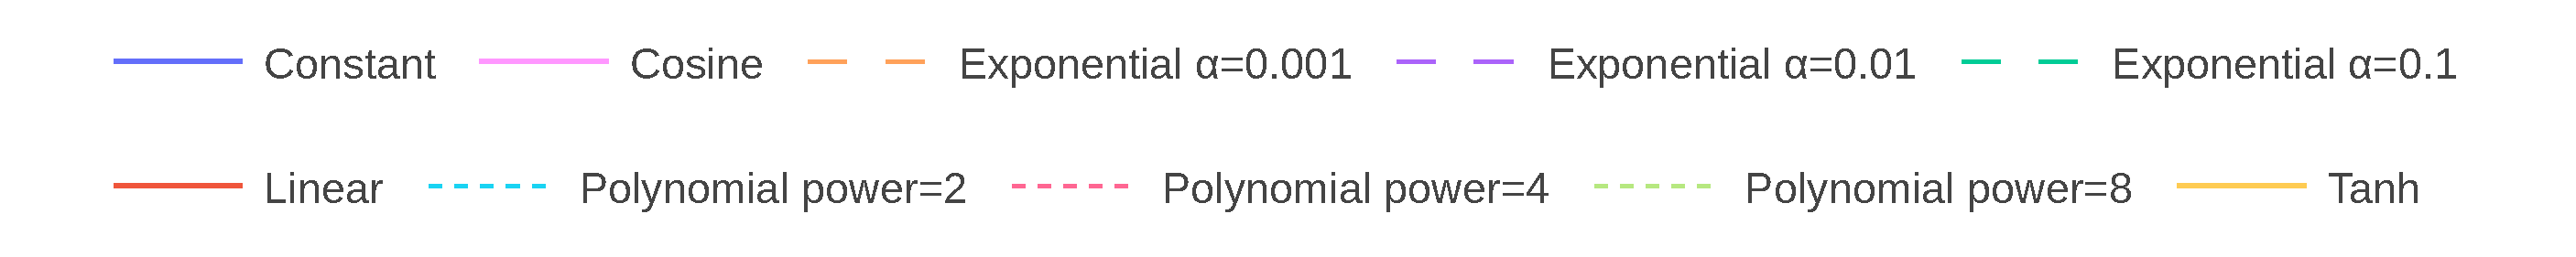
\includegraphics[scale=0.33]{figures/08/figures/noise_types_levels/rs_BBOBDistanceToOptimum_2_0.5_ei_rank_legend.pdf}
    \end{subfigure}
    \caption[Distance-based noise ranks on BBOB]{Mean ranks of regret resulting from running Bayesian optimisation with different distance-based noise functions over different noise levels. For all noise levels, constant noise 
    gives the best performance, with the margin increasing with the noise level.}
    \label{fig:ch08:dist_opt}
\end{figure}

\begin{figure}
    \centering
    \begin{subfigure}{0.24\textwidth}
        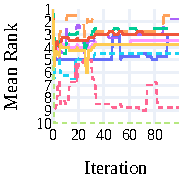
\includegraphics[]{figures/08/figures/noise_types_levels/rs_BBOBDistanceToOptimum_0.01_ei_rank_pd1.pdf}
        \caption{$N_\text{base}=0.01$}
    \end{subfigure}
    \begin{subfigure}{0.24\textwidth}
        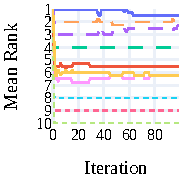
\includegraphics[]{figures/08/figures/noise_types_levels/rs_BBOBDistanceToOptimum_0.05_ei_rank_pd1.pdf}
        \caption{$N_\text{base}=0.05$}
    \end{subfigure}
    \begin{subfigure}{0.24\textwidth}
        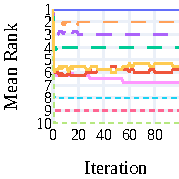
\includegraphics[]{figures/08/figures/noise_types_levels/rs_BBOBDistanceToOptimum_0.1_ei_rank_pd1.pdf}
        \caption{$N_\text{base}=0.1$}
    \end{subfigure}
    \begin{subfigure}{0.24\textwidth}
        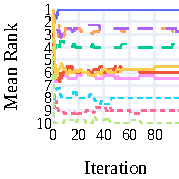
\includegraphics[]{figures/08/figures/noise_types_levels/rs_BBOBDistanceToOptimum_0.2_ei_rank_pd1.pdf}
        \caption{$N_\text{base}=0.2$}
    \end{subfigure}
    \begin{subfigure}{0.24\textwidth}
        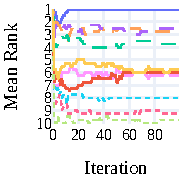
\includegraphics[]{figures/08/figures/noise_types_levels/rs_BBOBDistanceToOptimum_0.3_ei_rank_pd1.pdf}
        \caption{$N_\text{base}=0.3$}
    \end{subfigure}
    \begin{subfigure}{0.24\textwidth}
        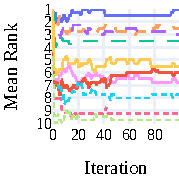
\includegraphics[]{figures/08/figures/noise_types_levels/rs_BBOBDistanceToOptimum_0.5_ei_rank_pd1.pdf}
        \caption{$N_\text{base}=0.5$}
    \end{subfigure}
    \begin{subfigure}{\textwidth}
        \centering
        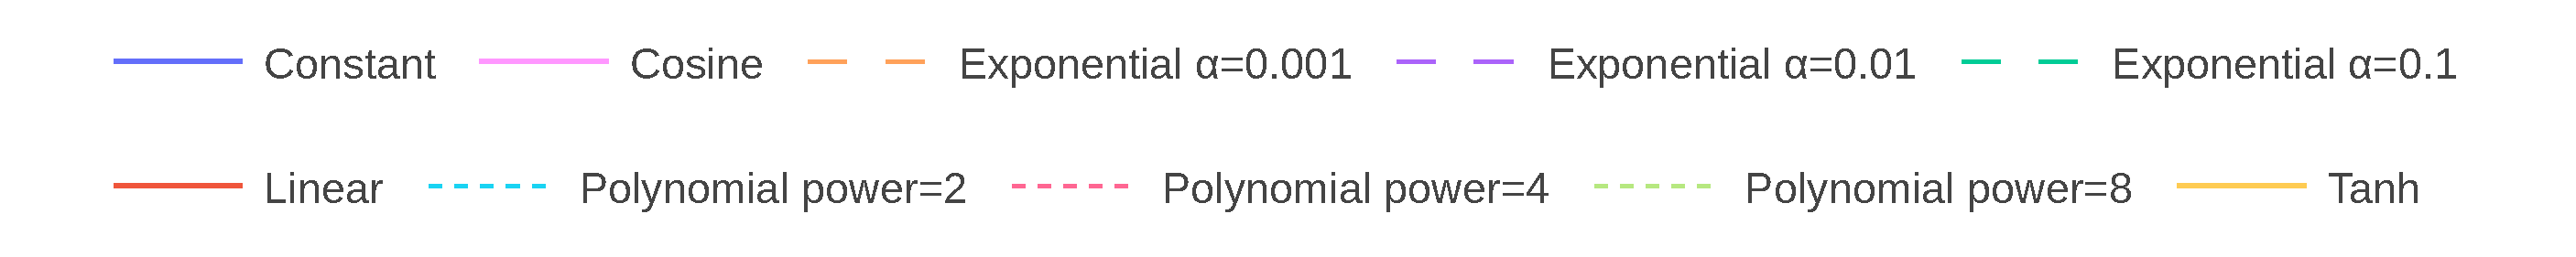
\includegraphics[scale=0.33]{figures/08/figures/noise_types_levels/rs_BBOBDistanceToOptimum_0.5_ei_rank_pd1_legend.pdf}
    \end{subfigure}
    \caption[Distance-based noise ranks on PD1]{Mean ranks of regret resulting from running Bayesian optimisation with different distance-based noise functions over different noise levels on the PD1 benchmark. Constant noise achieves best performance, unless the noise level is minimal.}
    \label{fig:ch08:dist_opt_pd1}
\end{figure}
Next, we evaluate noise functions based on the distance from the optimum. The results are presented in \cref{fig:ch08:dist_opt}. Similarly to the value-based noise functions, we look at all BBOB functions and use the optimisation with the EI acquisition function. Compared with value-based noise, distance-based noise exhibits markedly different behaviour with the noise schedules. Constant noise is consistently the strongest schedule; the performance gap widens with each increase in noise level. The exponential noise schedules follow the constant noise.

The same tendency appears on the PD1 benchmark (\cref{fig:ch08:dist_opt_pd1}), where distance-focused schedules are competitive only at the smallest noise settings and otherwise fail to match the more uniform alternatives. Notably, the constant noise baseline is the same for both value- and distance-based experiments. Since non-constant value-based noise functions outperform constant noise at low-to-moderate noise levels (\cref{fig:ch08:value_based}), while non-constant distance-based noise functions consistently underperform it (\cref{fig:ch08:dist_opt}), we can conclude that value-based noise allocation is generally preferable to distance-based allocation.

Taken together with the results from the previous sub-section, these results indicate that what is made accurate matters more than where: emphasising regions with good objective values is a safer strategy than emphasising geometric proximity to the final optimum.

\begin{figure}
    \centering
    \begin{subfigure}{0.24\textwidth}
        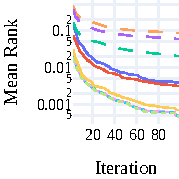
\includegraphics[]{figures/08/figures/conv/1_rs_BBOBDistanceToOptimum_2_0.01_ei_cov.pdf}
        \caption{F1 $N_\text{base}=0.01$}
    \end{subfigure}
    \begin{subfigure}{0.24\textwidth}
        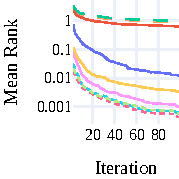
\includegraphics[]{figures/08/figures/conv/1_rs_BBOBDistanceToOptimum_2_0.05_ei_cov.pdf}
        \caption{F1 $N_\text{base}=0.05$}
    \end{subfigure}
    \begin{subfigure}{0.24\textwidth}
        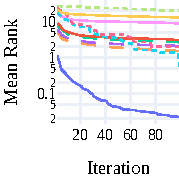
\includegraphics[]{figures/08/figures/conv/1_rs_BBOBDistanceToOptimum_2_0.1_ei_cov.pdf}
        \caption{F1 $N_\text{base}=0.1$}
    \end{subfigure}
    \begin{subfigure}{0.24\textwidth}
        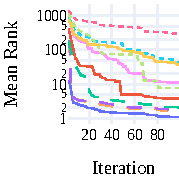
\includegraphics[]{figures/08/figures/conv/20_rs_BBOBDistanceToOptimum_2_0.01_ei_cov.pdf}
        \caption{F20 $N_\text{base}=0.01$}
    \end{subfigure}
    \begin{subfigure}{0.24\textwidth}
        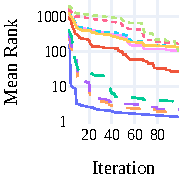
\includegraphics[]{figures/08/figures/conv/20_rs_BBOBDistanceToOptimum_2_0.05_ei_cov.pdf}
        \caption{F20 $N_\text{base}=0.05$}
    \end{subfigure}
    \begin{subfigure}{0.24\textwidth}
        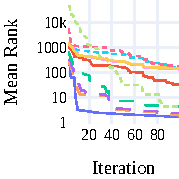
\includegraphics[]{figures/08/figures/conv/20_rs_BBOBDistanceToOptimum_2_0.1_ei_cov.pdf}
        \caption{F20 $N_\text{base}=0.1$}
    \end{subfigure}

    \begin{subfigure}[c]{1.0\textwidth}
        \centering

        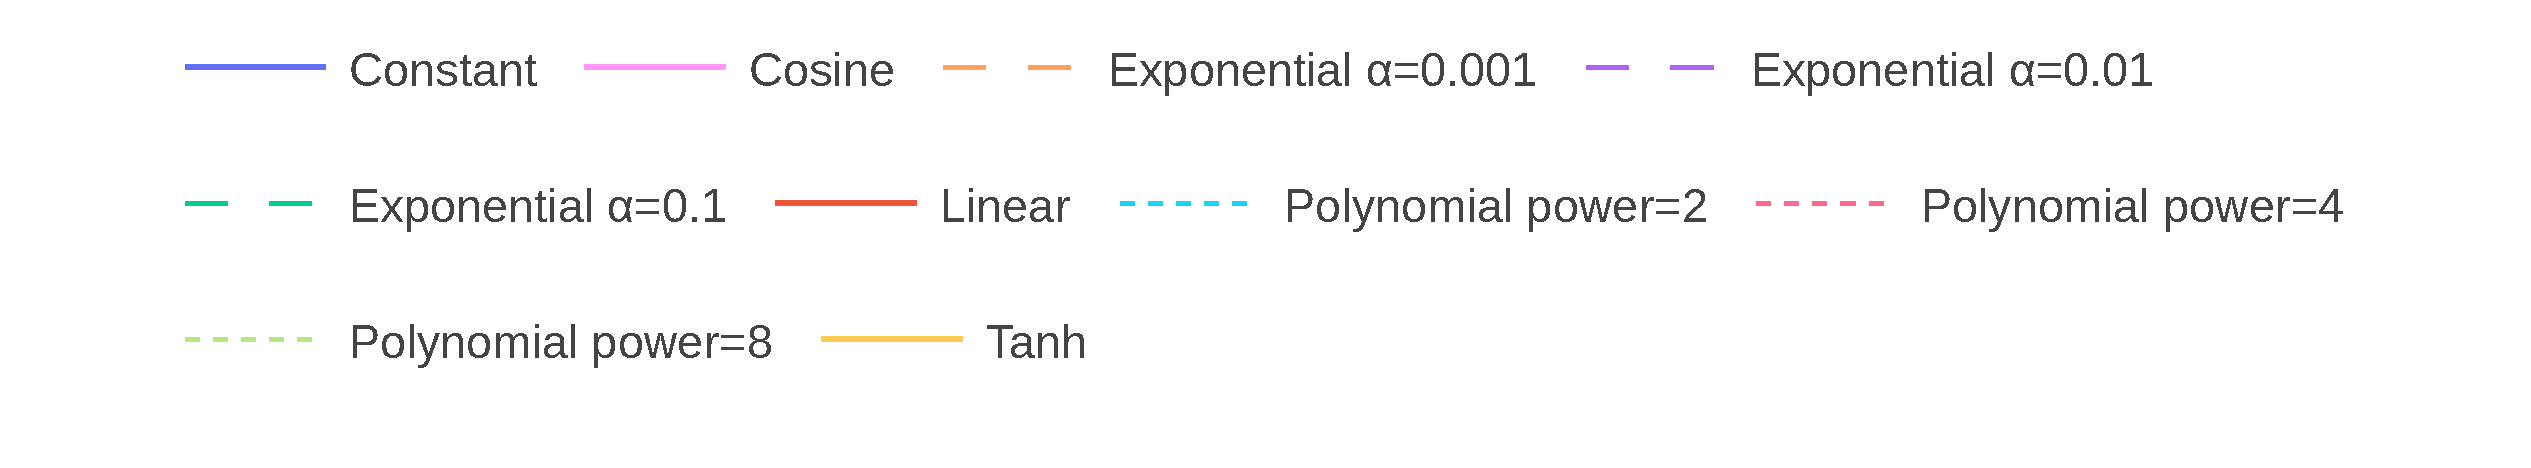
\includegraphics[scale=0.33]{figures/08/figures/conv/20_rs_BBOBDistanceToOptimum_2_0.1_ei_cov_legend.pdf}


    \end{subfigure}
    \caption[Convergence plots with distance-based noise]{Convergence plots of BBOB functions 1 (a-c) and 20 (d-f) with noise levels ($0.01, 0.05, 0.1$), different noise schedules using distance-based noise. On function 1 and lower noise levels, it is better to be accurate around the optimum. For function 20, constant noise dominates, followed by more benign noise functions that give only modest advantage to solutions around the optimum.}
    \label{fig:ch08:conv_sample}
\end{figure}

We show convergence plots of BBOB functions 1 and 20 with different noise functions and levels in \cref{fig:ch08:conv_sample}. These results use distance-based noise. Function 1 is the Sphere function, a simple unimodal function with no local optima. Function 20, on the other hand, is the Schwefel function, which has multiple local optima, including some that are relatively close in value to the optimum but far from it in distance.

For function 1 with low noise levels ($0.01$ and $0.05$), the polynomial noise functions perform very well, similar to the value-based case. However, when the noise level increases, constant noise becomes optimal, as the penalty assigned to points far from the optimum becomes disproportionately large. For function 20, constant noise is consistently the best, followed by benign noise functions that give only a small area around the optimum good values and therefore impose only a small penalty on distant solutions.
The trajectories make the difference between the two functions particularly clear: on F1, several schedules remain competitive for a substantial part of the run and only separate clearly as the noise level increases, whereas on F20 the constant schedule establishes an advantage early and maintains it throughout. This is consistent with the intuition that multimodality makes distance-based inaccuracies more damaging, because the optimiser is more likely to be drawn toward distant but deceptively attractive regions.

These results challenge the common assumption that being accurate around the optimum is sufficient for a good surrogate. Furthermore, being accurate only around the optimum, and not around other areas of good value, can be seen as providing an additional ``oracle'' hint. However, in practice, the optimiser confuses poorly predicted solutions with good ones, while neglecting the real optimum.



\subsection{Comparing value-based and distance-based noise within each schedule}
\begin{figure}[!htbp]
    \centering
    \begin{subfigure}{0.19\textwidth}
        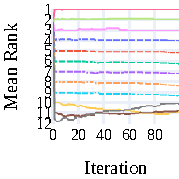
\includegraphics[]{figures/08/figures/noise_type_comp/rs_linear_2_ei_rank.pdf}
        \caption{Linear}
    \end{subfigure}
    \begin{subfigure}{0.19\textwidth}
        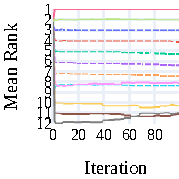
\includegraphics[]{figures/08/figures/noise_type_comp/rs_exp_0.1_2_ei_rank.pdf}
        \caption{Exp 0.1}
    \end{subfigure}
    \begin{subfigure}{0.19\textwidth}
        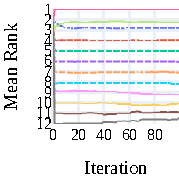
\includegraphics[]{figures/08/figures/noise_type_comp/rs_exp_0.01_2_ei_rank.pdf}
        \caption{Exp 0.01}
    \end{subfigure}
    \begin{subfigure}{0.19\textwidth}
        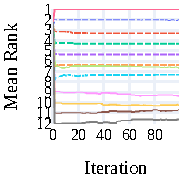
\includegraphics[]{figures/08/figures/noise_type_comp/rs_exp_0.001_2_ei_rank.pdf}
        \caption{Exp 0.001}
    \end{subfigure}
    \begin{subfigure}{0.19\textwidth}
        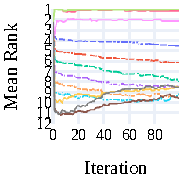
\includegraphics[]{figures/08/figures/noise_type_comp/rs_poly_2_2_ei_rank.pdf}
        \caption{Poly 2}
    \end{subfigure}
    \begin{subfigure}{0.19\textwidth}
        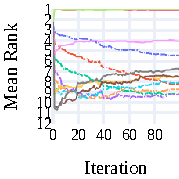
\includegraphics[]{figures/08/figures/noise_type_comp/rs_poly_4_2_ei_rank.pdf}
        \caption{Poly 4}
    \end{subfigure}
    \begin{subfigure}{0.19\textwidth}
        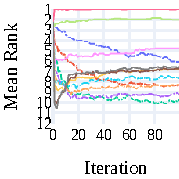
\includegraphics[]{figures/08/figures/noise_type_comp/rs_poly_8_2_ei_rank.pdf}
        \caption{Poly 8}
    \end{subfigure}
    \begin{subfigure}{0.19\textwidth}
        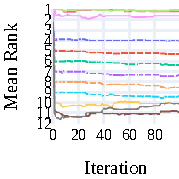
\includegraphics[]{figures/08/figures/noise_type_comp/rs_cosine_2_ei_rank.pdf}
        \caption{Cosine}
    \end{subfigure}
    \begin{subfigure}{0.19\textwidth}
        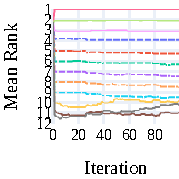
\includegraphics[]{figures/08/figures/noise_type_comp/rs_tanh_2_ei_rank.pdf}
        \caption{TanH}
    \end{subfigure}
    \begin{subfigure}{\textwidth}
        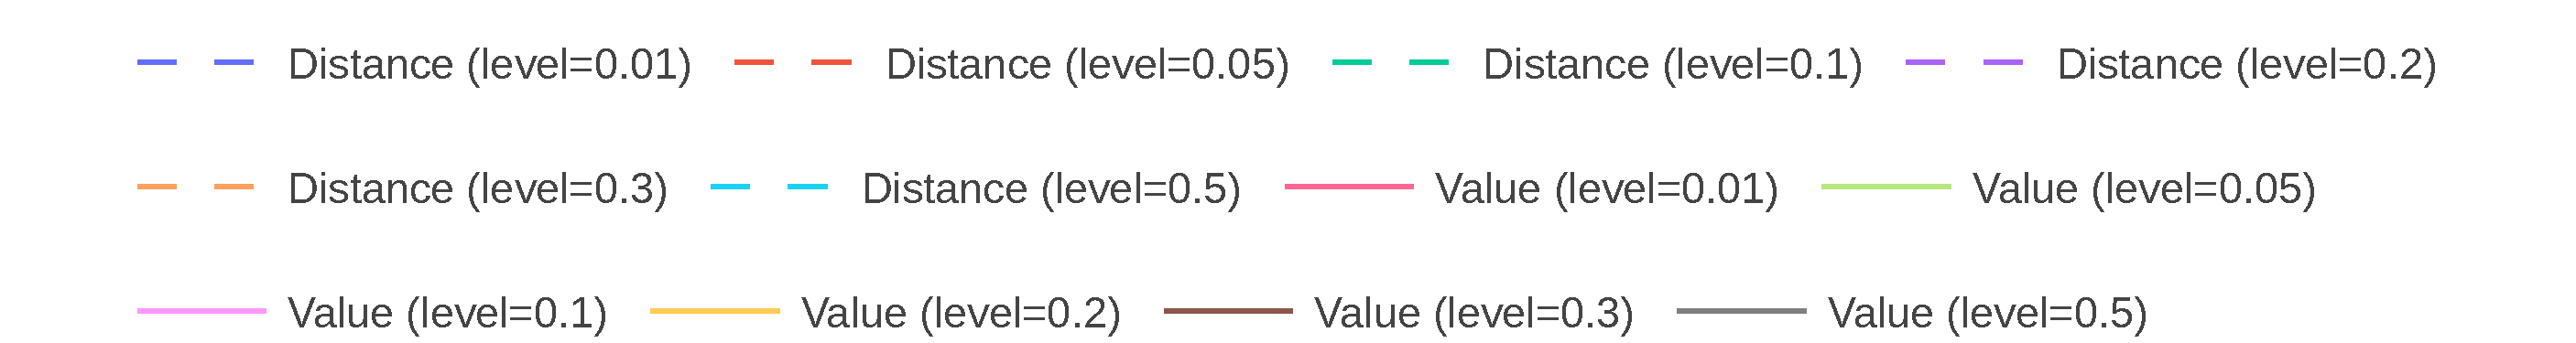
\includegraphics[scale=0.33]{figures/08/figures/noise_type_comp/rs_tanh_2_ei_rank_legend.pdf}

    \end{subfigure}
    \caption[Noise type and level comparison on BBOB]{Mean ranks of the regret resulting from running Bayesian optimisation with different noise types and levels. Each plot represents one noise function. For polynomial noise functions, value-based noise is superior to distance-based noise.}
    \label{fig:ch08:function_types}
\end{figure}


We compare value-based and distance-based noise within each schedule family. In \cref{fig:ch08:function_types,fig:ch08:function_types_pd1}, each sub-figure shows one noise schedule, with lines for value-based and distance-based variants across all tested noise levels. This experiment was conducted using EI as the acquisition function and random search for acquisition function optimisation on dimension 2.

\begin{figure}[!htbp]
    \centering
    \begin{subfigure}{0.19\textwidth}
        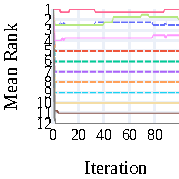
\includegraphics[]{figures/08/figures/noise_type_comp/rs_linear_ei_rank_pd1.pdf}
        \caption{Linear}
    \end{subfigure}
    \begin{subfigure}{0.19\textwidth}
        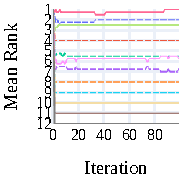
\includegraphics[]{figures/08/figures/noise_type_comp/rs_exp_0.1_ei_rank_pd1.pdf}
        \caption{Exp 0.1}
    \end{subfigure}
    \begin{subfigure}{0.19\textwidth}
        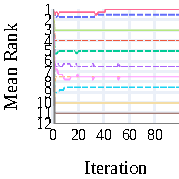
\includegraphics[]{figures/08/figures/noise_type_comp/rs_exp_0.01_ei_rank_pd1.pdf}
        \caption{Exp 0.01}
    \end{subfigure}
    \begin{subfigure}{0.19\textwidth}
        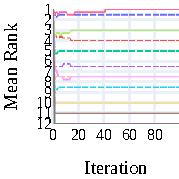
\includegraphics[]{figures/08/figures/noise_type_comp/rs_exp_0.001_ei_rank_pd1.pdf}
        \caption{Exp 0.001}
    \end{subfigure}
    \begin{subfigure}{0.19\textwidth}
        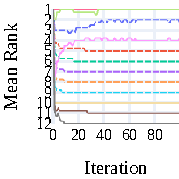
\includegraphics[]{figures/08/figures/noise_type_comp/rs_poly_2_ei_rank_pd1.pdf}
        \caption{Poly 2}
    \end{subfigure}
    \begin{subfigure}{0.19\textwidth}
        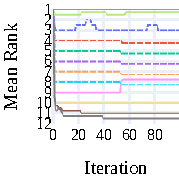
\includegraphics[]{figures/08/figures/noise_type_comp/rs_poly_4_ei_rank_pd1.pdf}
        \caption{Poly 4}
    \end{subfigure}
    \begin{subfigure}{0.19\textwidth}
        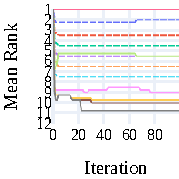
\includegraphics[]{figures/08/figures/noise_type_comp/rs_poly_8_ei_rank_pd1.pdf}
        \caption{Poly 8}
    \end{subfigure}
    \begin{subfigure}{0.19\textwidth}
        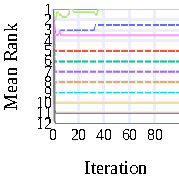
\includegraphics[]{figures/08/figures/noise_type_comp/rs_cosine_ei_rank_pd1.pdf}
        \caption{Cosine}
    \end{subfigure}
    \begin{subfigure}{0.19\textwidth}
        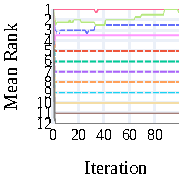
\includegraphics[]{figures/08/figures/noise_type_comp/rs_tanh_ei_rank_pd1.pdf}
        \caption{TanH}
    \end{subfigure}
    \begin{subfigure}{\textwidth}
        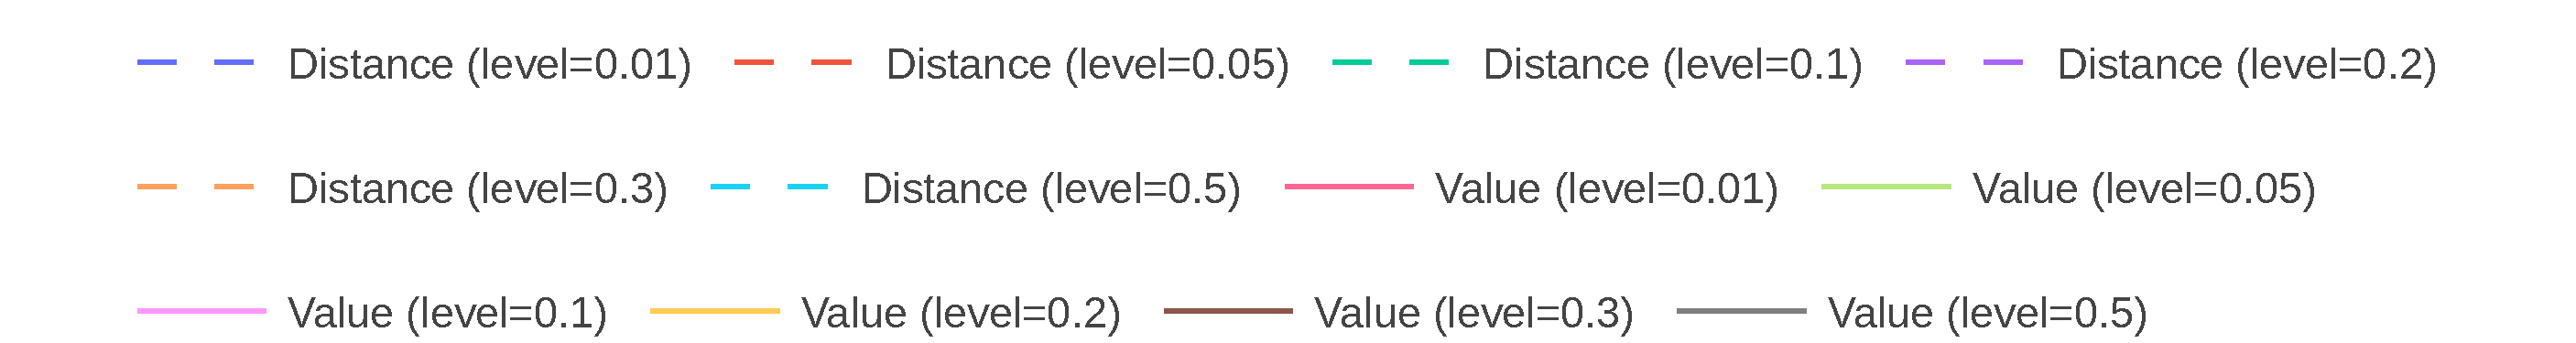
\includegraphics[scale=0.33]{figures/08/figures/noise_type_comp/rs_tanh_ei_rank_pd1_legend.pdf}

    \end{subfigure}
    \caption[Noise type and level comparison on PD1]{Mean ranks of regret resulting from evaluating different noise types and levels on the PD1 benchmark. Each plot represents a specific noise function, comparing its value-based and distance-based variants across noise levels.}
    \label{fig:ch08:function_types_pd1}
\end{figure}


\cref{fig:ch08:function_types,fig:ch08:function_types_pd1} show that for smooth noise functions such as linear, cosine and tanh, the value-based variant is superior, but the distance-based variant with low noise remains competitive; in contrast, sharper families (notably higher-order polynomial and steep exponential variants) are more sensitive and expose clearer differences between the two formulations. This is consistent with the idea that steep schedules amplify inductive bias: if the bias is aligned with objective quality, performance can improve, but if aligned only with distance, the optimiser is more easily led astray.

\subsection{Different acquisition functions}
We now check whether different acquisition functions require a different accuracy focus from the surrogate model. We evaluate PI and LCB in addition to the EI results presented earlier, using a noise level of $0.1$ and the 24 BBOB functions on dimension 2.
The results are shown in \cref{fig:ch08:diff_acqs}.


\begin{figure}
    \centering
    \begin{subfigure}[c]{0.24\textwidth}
        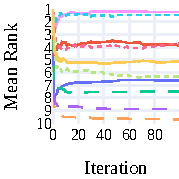
\includegraphics[]{figures/08/figures/noise_types_levels/rs_BBOBValueBased_2_0.1_pi_rank.pdf}
        \caption{PI}
    \end{subfigure}
    \begin{subfigure}[c]{0.24\textwidth}
        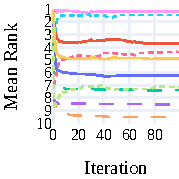
\includegraphics[]{figures/08/figures/noise_types_levels/rs_BBOBValueBased_2_0.1_lcb_rank.pdf}
        \caption{LCB}
    \end{subfigure}
    \hspace{0.5cm}
    \begin{subfigure}[c]{\textwidth} 
        \centering
        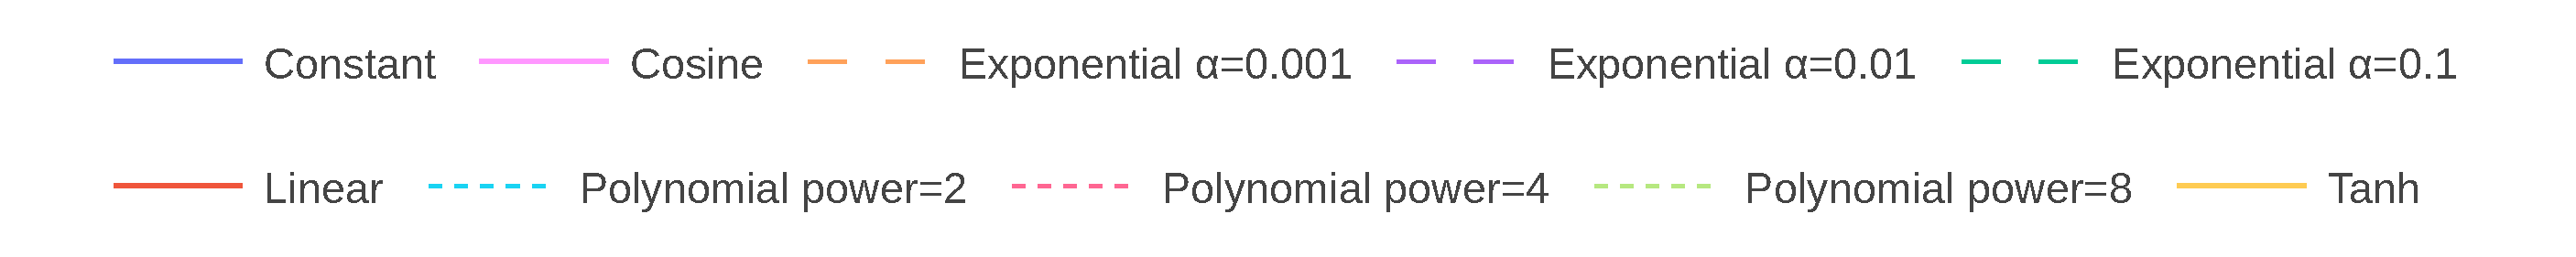
\includegraphics[scale=0.33]{figures/08/figures/noise_types_levels/rs_BBOBValueBased_2_0.1_lcb_rank_legend.pdf}
    \end{subfigure}
    \caption[Acquisition function comparison on BBOB]{Mean ranks of regret resulting from running Bayesian optimisation with value-based noise functions with different acquisition functions and noise level of $0.1$. (a) PI. (b) LCB. The best performing noise functions remain similar to using EI as an acquisition.}
    \label{fig:ch08:diff_acqs}
\end{figure}

\begin{figure}
    \centering
    \begin{subfigure}[c]{0.24\textwidth}
        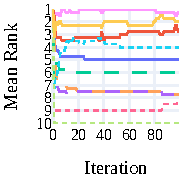
\includegraphics[]{figures/08/figures/noise_types_levels/rs_BBOBValueBased_0.1_pi_rank_pd1.pdf}
        \caption{PI}
    \end{subfigure}
    \begin{subfigure}[c]{0.24\textwidth}
        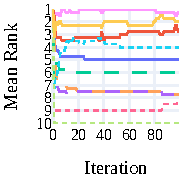
\includegraphics[]{figures/08/figures/noise_types_levels/rs_BBOBValueBased_0.1_lcb_rank_pd1.pdf}
        \caption{LCB}
    \end{subfigure}
    \hspace{0.5cm}
    \begin{subfigure}[c]{\textwidth}
        \centering
        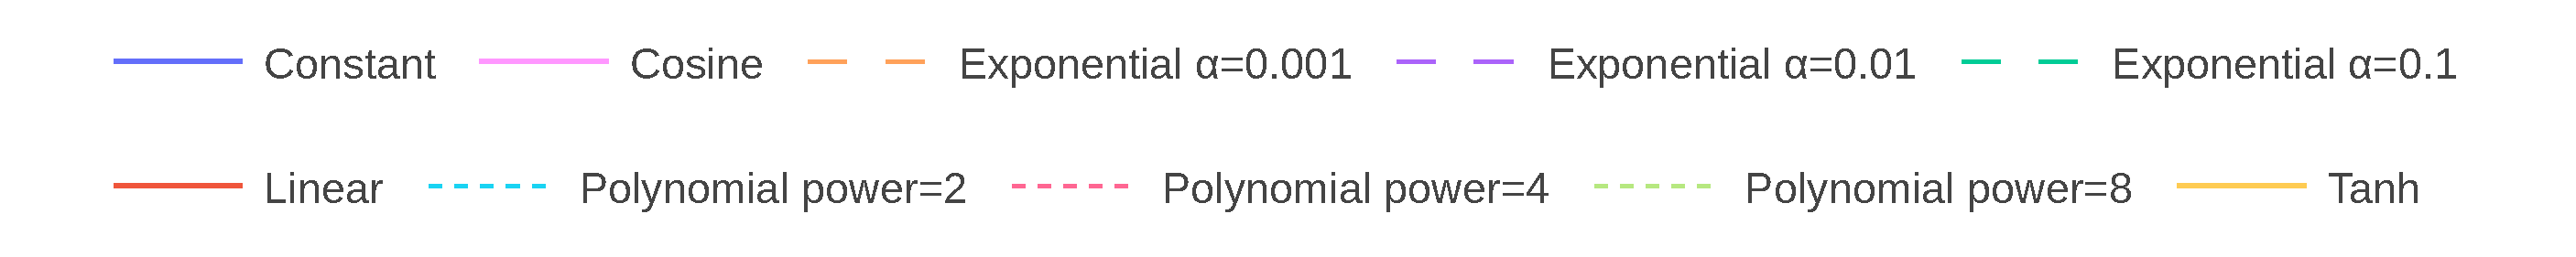
\includegraphics[scale=0.33]{figures/08/figures/noise_types_levels/rs_BBOBValueBased_0.1_lcb_rank_pd1_legend.pdf}
    \end{subfigure}
    \caption[Acquisition function comparison on PD1]{Mean ranks of regret on the PD1 benchmark using value-based noise with (a) PI and (b) LCB acquisition functions at a noise level of $0.1$. The relative performance of the noise functions remains consistent with EI.}
    \label{fig:ch08:diff_acqs_pd1}
\end{figure}

The rankings under PI and LCB (\cref{fig:ch08:diff_acqs,fig:ch08:diff_acqs_pd1}) closely mirror the EI case, with only minor swaps among similarly performing schedules. In particular, the cosine and polynomial schedules that perform well under EI remain among the top schedules under PI and LCB, whereas constant noise occupies a similar mid-range position. PI, being a greedier acquisition function, might be expected to be more sensitive to prediction accuracy near the incumbent, but we do not observe a qualitatively different pattern. This indicates that our conclusions about useful noise allocation are not tied to a specific acquisition criterion.

\subsection{Different acquisition optimisers}
In the next step, we also check whether different acquisition function optimisers are required. We compare local and random search as acquisition optimisers on BBOB in \cref{fig:ch08:acq_opts}.
\begin{figure}
    \centering
    \begin{subfigure}[c]{0.24\textwidth}
        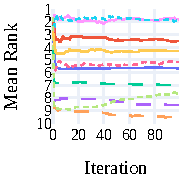
\includegraphics[]{figures/08/figures/noise_types_levels/default_BBOBValueBased_2_0.1_ei_rank.pdf}

    \end{subfigure}
    \hspace{0.5cm}
    \begin{subfigure}[c]{\textwidth}
        \centering

        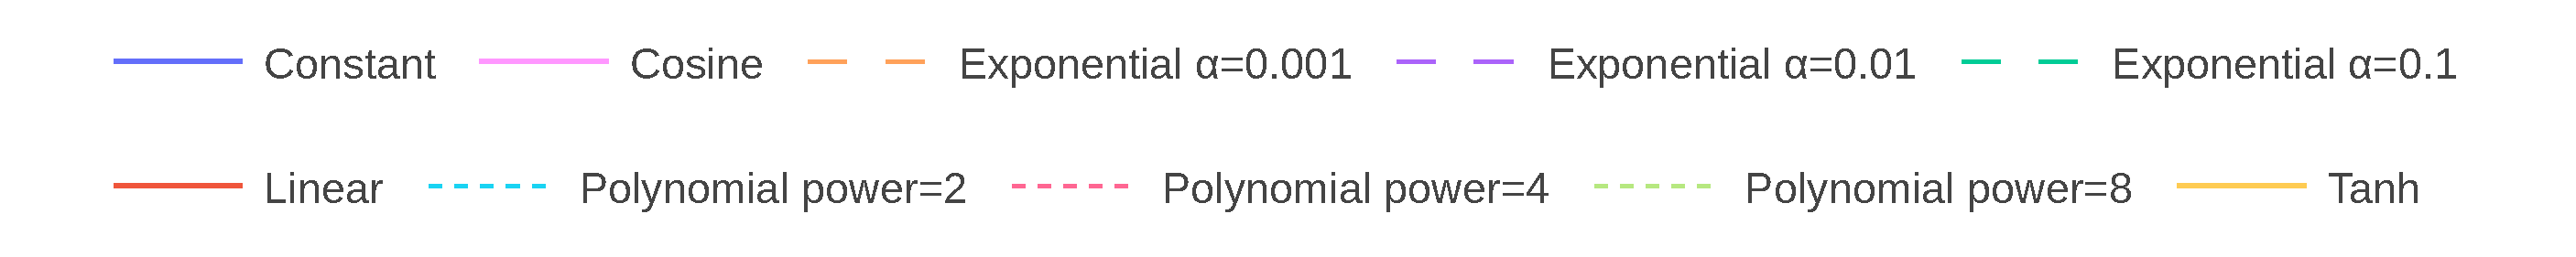
\includegraphics[scale=0.33]{figures/08/figures/noise_types_levels/default_BBOBValueBased_2_0.1_ei_rank_legend.pdf}


    \end{subfigure}
    \caption[Local search optimisation comparison on BBOB]{Mean ranks of regret resulting from running Bayesian optimisation with value-based noise functions using different acquisition function optimisers: local search and random search, at a noise level of $0.1$. The best-performing noise functions remain similar to the random search case.}
    \label{fig:ch08:acq_opts}
\end{figure}

\begin{figure}
    \centering
    \begin{subfigure}[c]{0.24\textwidth}
        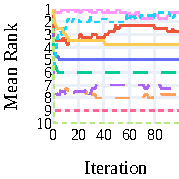
\includegraphics[]{figures/08/figures/noise_types_levels/default_BBOBValueBased_0.1_ei_rank_pd1.pdf}
    \end{subfigure}
    \hspace{0.5cm}
    \begin{subfigure}[c]{\textwidth}
        \centering
        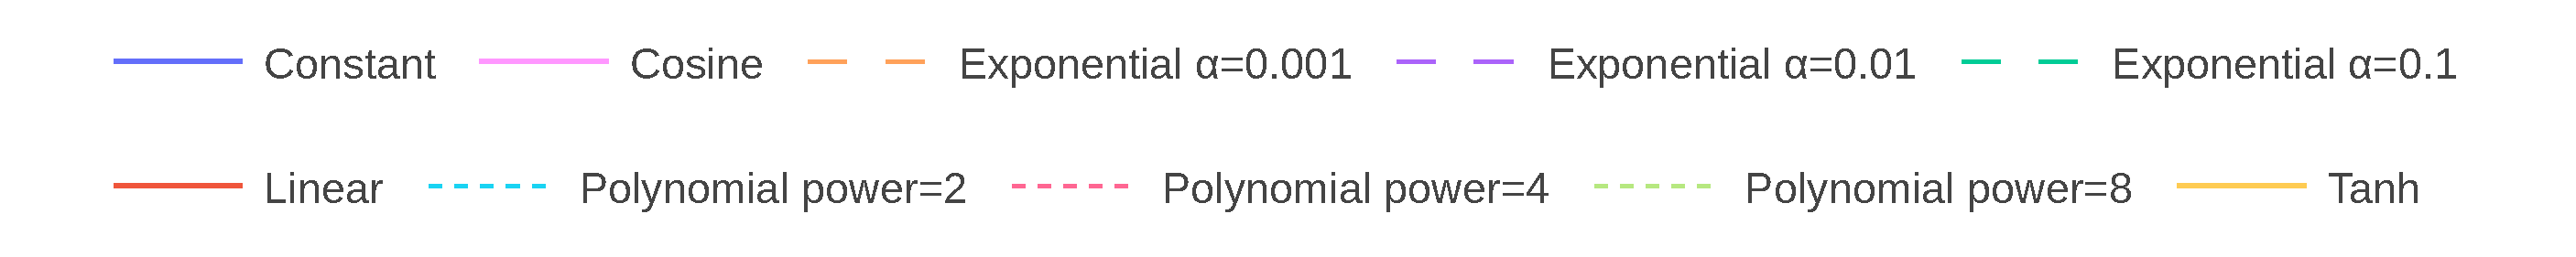
\includegraphics[scale=0.33]{figures/08/figures/noise_types_levels/default_BBOBValueBased_0.1_ei_rank_pd1_legend.pdf}
    \end{subfigure}
    \caption[Local search optimisation comparison on PD1]{Mean ranks of regret on the PD1 benchmark using value-based noise and local search for acquisition function optimisation at a noise level of $0.1$.}
    \label{fig:ch08:acq_opts_pd1}
\end{figure}

Changing the acquisition optimiser from random search to local search (\cref{fig:ch08:acq_opts,fig:ch08:acq_opts_pd1}) leaves the qualitative ordering largely unchanged. In particular, schedules that perform well with random search remain competitive with local search, indicating that the observed trends are driven primarily by surrogate-noise design rather than by the particular search dynamics of the optimiser. We note that \cref{fig:ch08:acq_opts_pd1} shows results only with local search on PD1, as the random search baseline is already reported in \cref{fig:ch08:value_based_pd1}.

\subsection{Dimensionalities}
We check whether our results hold across different dimensionalities of the BBOB suite. We present results for value-based noise functions with EI as the acquisition function and a noise level of $0.1$, on dimensions $4$ and $8$, in \cref{fig:ch08:dims}. 
\begin{figure}
    \centering
    \begin{subfigure}[c]{0.24\textwidth}
        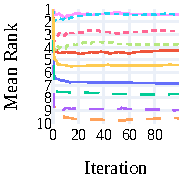
\includegraphics[]{figures/08/figures/noise_types_levels/rs_BBOBValueBased_4_0.1_ei_rank.pdf}
        \caption{4}
    \end{subfigure}
    \begin{subfigure}[c]{0.24\textwidth}
        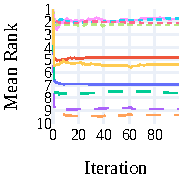
\includegraphics[]{figures/08/figures/noise_types_levels/rs_BBOBValueBased_8_0.1_ei_rank.pdf}
        \caption{8}
    \end{subfigure}
    \hspace{0.5cm}
    \begin{subfigure}[c]{\textwidth}
        \centering 
        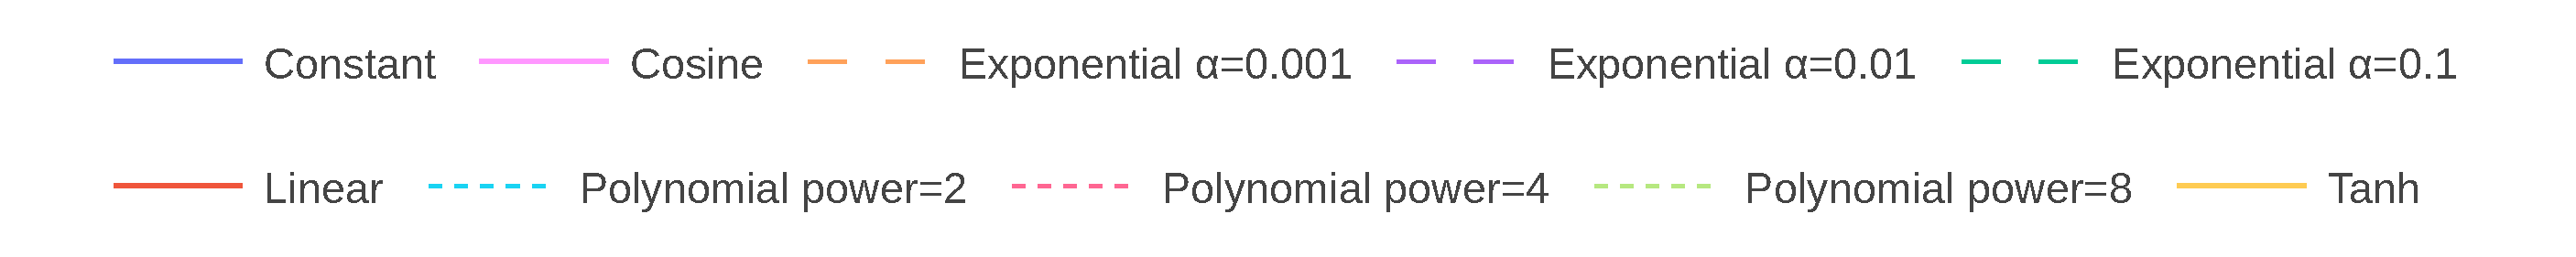
\includegraphics[scale=0.33]{figures/08/figures/noise_types_levels/rs_BBOBValueBased_8_0.1_ei_rank_legend.pdf}
    \end{subfigure}
    \caption[Combined noise analysis on BBOB]{Mean ranks of resulting regrets of running Bayesian optimisation with EI as an acquisition function with different value-based noise functions over different noise levels. With a noise level of $0.1$ on dimensions 4 and 8. With higher dimensions, more noise functions perform well. However, constant noise performs worse than other noise levels for both cases.}
    \label{fig:ch08:dims}
\end{figure}

\cref{fig:ch08:dims} suggests that increasing dimensionality compresses differences among the better non-constant schedules, but does not reverse the main conclusion. Several value-based schedules remain strong in both $d=4$ and $d=8$, while constant noise is still typically among the weaker options. This indicates that the benefit of allocating fidelity by objective quality is not limited to the lowest-dimensional setting tested.

\subsection{Summary of experimental findings}
Taken together, the experiments indicate a consistent pattern. In a low-to-moderate noise regime, \gls{bo} benefits from non-uniform, value-based fidelity allocation; in a high-noise regime, the advantage of strong non-uniformity shrinks and simpler schedules become more competitive. Importantly, this pattern remains visible when changing acquisition function, acquisition optimiser, and dimensionality, suggesting that it reflects a structural property of how \gls{bo} reacts to surrogate distortion rather than a setup-specific artifact.
We also observed that in general, value-based noise functions are superior to distance based ones.

The convergence comparison on F1 versus F20 further suggests that landscape structure modulates this trade-off. On smoother landscapes, non-uniform schedules can remain beneficial for longer. Other the other hand, on multimodal landscapes, schedules that heavily degrade distant points are riskier because the optimiser encounters more suboptimal-but-competitive regions that can be over-promoted by distorted predictions.

}
\section{Comparison to real-world surrogate models}
\begin{figure}[tbp]
    \centering
    \begin{subfigure}{0.25\textwidth}
        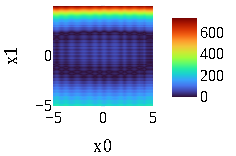
\includegraphics[]{figures/08/figures/contours/gp_10.pdf}
        \caption{10}
    \end{subfigure}
    \begin{subfigure}{0.25\textwidth}
        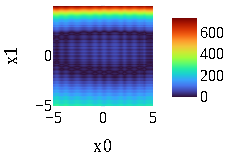
\includegraphics[]{figures/08/figures/contours/gp_25.pdf}
        \caption{25}
    \end{subfigure}
    \begin{subfigure}{0.25\textwidth}
        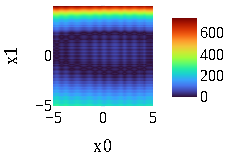
\includegraphics[]{figures/08/figures/contours/gp_50.pdf}
        \caption{50}
    \end{subfigure}
    \begin{subfigure}{0.25\textwidth}
        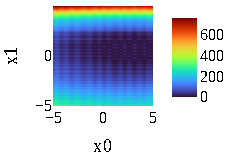
\includegraphics[]{figures/08/figures/contours/gp_100.pdf}
        \caption{100}
    \end{subfigure}
    \begin{subfigure}{0.25\textwidth}
        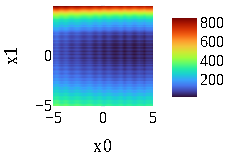
\includegraphics[]{figures/08/figures/contours/ground_truth.pdf}
        \caption{Ground truth}
    \end{subfigure}
    \caption[GP error analysis on BBOB F3]{Error of GP trained on different subsets of solutions from a trajectory of \gls{bo} on BBOB F3 (a-d). (e) ground truth values of the function. When the optimisation progresses, better predictions are made in high-performance regions, at the expense of low-performance regions.}
    \label{fig:ch08:gps_accs}
\end{figure}

\changed{Following the noisy-oracle experiments, we examine how real surrogate models behave on an actual \gls{bo} trajectory. The goal of this section is not to reproduce the earlier controlled setup exactly, but to check whether the qualitative pattern suggested by the noisy oracle can also be seen in standard surrogate models.}
\changed{We use BBOB function 3 in dimension 2 because it has multiple local optima while still being easy to visualise. We run SMAC3~\cite{LinEtAl22} for 100 evaluations and then train a Gaussian process on the first 10, 25, 50 and 100 solutions from the trajectory. The Gaussian process uses the default SMAC3 settings (\emph{i.e.}, a Matern kernel optimized with L-BFGS-B). We evaluate its absolute error on a grid of 10\,000 points over the full landscape. Results from the analogous experiment with random forest are shown next.}

\changed{The results are presented in \cref{fig:ch08:gps_accs}, together with the ground-truth function values. Early in the optimisation, the Gaussian process is already relatively accurate in some high-performance regions, but not necessarily exactly at the optimum. As the search progresses and more samples are gathered around the optimum, the error decreases in that region, while accuracy may deteriorate in parts of the landscape that are far away (for example around $x_2=-2.5$). This pattern does not prove that the GP follows the noisy-oracle mechanism exactly, but it is qualitatively consistent with our earlier observation that BO benefits when the surrogate allocates more accuracy to regions with good objective values than to uniformly poor regions.}


\changed{\cref{fig:ch08:rfs_accs} shows the corresponding behaviour for random forest. We again observe that the model is more accurate in regions with better objective values, similarly to the GP. Compared to the GP, however, the random forest tends to concentrate its lower-error predictions in smaller regions. This makes the random-forest result consistent with the same qualitative story, while also illustrating that different surrogate classes may realize this behaviour in different geometric ways.}
\begin{figure}[tbp]
    \centering
    \begin{subfigure}{0.25\textwidth}
        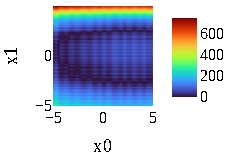
\includegraphics[]{figures/08/figures/contours/rf_10.pdf}
        \caption{10}
    \end{subfigure}
    \begin{subfigure}{0.25\textwidth}
        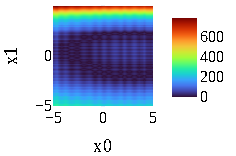
\includegraphics[]{figures/08/figures/contours/rf_25.pdf}
        \caption{25}
    \end{subfigure}
    \begin{subfigure}{0.25\textwidth}
        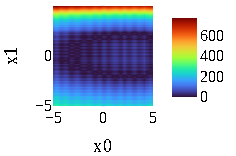
\includegraphics[]{figures/08/figures/contours/rf_50.pdf}
        \caption{50}
    \end{subfigure}
    \begin{subfigure}{0.25\textwidth}
        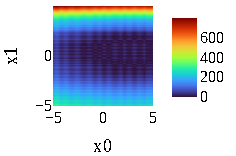
\includegraphics[]{figures/08/figures/contours/rf_100.pdf}
        \caption{100}
    \end{subfigure}
    \begin{subfigure}{0.25\textwidth}
        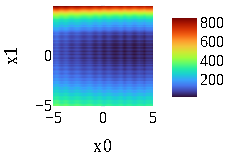
\includegraphics[]{figures/08/figures/contours/ground_truth.pdf}
        \caption{Ground truth}
    \end{subfigure}
    \caption[Random forest error analysis on BBOB F3]{Error of random forest trained on different subsets of solutions from a trajectory of \gls{bo} on BBOB F3 (a-d). (e) ground truth values of the function. When the optimisation progresses, better predictions are made in high-performance regions, at the expense of low-performance regions.}
    \label{fig:ch08:rfs_accs}
\end{figure}

\section{Theoretical analysis}
\changed{Our empirical results with the noisy oracle (e.g., \cref{fig:ch08:value_based,fig:ch08:dist_opt}) suggest that substantial surrogate-model inaccuracy can be detrimental, especially when it makes suboptimal points appear unrealistically attractive. In this section, we study a deterministic analogue of this phenomenon to better understand when such misleading behaviour can occur.

We provide a theoretical analysis of a deterministic version of the noisy oracle surrogate model. The purpose of this analysis is to derive simple, conditions under which the acquisition function prefers a suboptimal point to the optimum because the surrogate prediction is distorted.

We note that the choice to analyse a deterministic surrogate rather than the stochastic oracle used in the experiments for two reasons. First, a stochastic oracle produces different predictions at each query, so the event ``the acquisition function is misled'' becomes a probabilistic statement that depends on the joint distribution of all noise draws across all evaluated candidates within an iteration. Deriving tight, interpretable bounds in this setting would require additional assumptions about the number of candidates, the correlation structure of queries, and the acquisition optimiser search strategy, which would obscure the core message. Second, we define the deterministic model represents a pessimistic, worst-case, scenario in which the surrogate consistently predicts values that are better than the truth by exactly the assigned noise magnitude. If the acquisition function can be misled under this deterministic bias, then it can certainly be misled by the stochastic oracle whenever a noise draw happens to produce a similarly large deviation, which occurs with non-negligible probability when $N(x_L)$ is large. In other words, the deterministic thresholds serve as sufficient conditions for the possibility of misleading behaviour under the stochastic oracle as they identify the noise magnitudes at which the risk of being misled becomes structurally unavoidable rather than merely a rare tail event.
\subsection{General definitions}
\label{sec:ch08:gen_defs}
\changed{We define $x_L\in \sR^n$ as a suboptimal point such that $f(x_L) = f(x^*) + l$, where $l > 0$. Thus, $l$ measures the objective gap between the optimum and the suboptimal point.}


\changed{At the optimum, the noise for the mean prediction is minimal, as $\hat{N}(x^*)=0$ and therefore $N(x^*)=N_\text{min}$. For the theoretical analysis, we consider a deterministic surrogate that always predicts values that are better than the truth by an amount equal to the assigned noise. This gives a pessimistic but easy-to-analyse model of how biased predictions can mislead \gls{bo}. Therefore, the model predicts:}
\begin{equation*}
    \mu_S(x^*) = f(x^*) - N_{\min}
\end{equation*}
\begin{equation*}
    \sigma_S(x^*) = \sigma(x^*)
\end{equation*}
where $N_{\min} > 0$.

\changed{At the suboptimal point $x_L$, the surrogate model also predicts a value that is better than the truth. Therefore, the model predicts:}
\begin{equation*}
    \mu_S(x_L) = f(x_L) - N(x_L) = f(x^*) + l - N(x_L)
\end{equation*}
\begin{equation*}
    \sigma_S(x_L) = \sigma(x_L)
\end{equation*}
where $N(x_L) > 0$, as we assume the model strictly predicts lower values for $\mu_S(x_L)$ than the actual objective values.

\subsection{Expected Improvement}
We define $I_{x^*} = f(x_{best}) - f(x^*)$ as the difference between the incumbent solution and the optimum. We note that $I_{x^*} \ge 0$.

\begin{theorem}
if
\begin{equation*}
    N(x_L) > I_{x^*} + l + 2 \cdot N_{\min} + 0.798 \cdot \sigma(x^*)
\end{equation*}
then the EI acquisition function is guaranteed to be misled.
\end{theorem}

\begin{proof}
We first evaluate the expected improvement at the optimum $x^*$. We calculate the $z$ value at $x^*$, denoted as $z_{x^*}$:
\begin{equation}
    \label{eq:ch08:z_xstar}
    z_{x^*} = \frac{f(x_{best}) - \mu_S(x^*)}{\sigma_S(x^*)} = \frac{f(x_{best}) - f(x^*)+ N_{\min}}{\sigma(x^*)}=\frac{I_{x^*} + N_{\min}}{\sigma(x^*)}
\end{equation}
Since $I_{x^*},N_{\min},\sigma(x^*) \ge 0$, we have $z_{x^*} \ge 0$, and therefore $\Phi(z_{x^*}) \le 1$ and $\phi(z_{x^*}) \le 0.399$. This gives the upper bound for the expected improvement at the optimum:
\begin{equation}
    \label{eq:ch08:EI_star_bound}
    \mathrm{EI}(x^*) \le I_{x^*} + N_{\min} + 0.399 \cdot \sigma(x^*)
\end{equation}

Next, we evaluate the expected improvement at the suboptimal solution $x_L$. We first calculate the $z$ value at $x_L$:
\begin{equation}
    \label{eq:ch08:z_xl}
    z_{x_L} = \frac{f(x_{best}) - \mu_S(x_L)}{\sigma_S(x_L)}=\frac{f(x_{best}) - f(x^*) - l + N(x_L)}{\sigma(x_L)}=\frac{I_{x^*}-l+N(x_L)}{\sigma(x_L)}
\end{equation}

The acquisition function is misled if $\mathrm{EI}(x_L) > \mathrm{EI}(x^*)$. We analyse a sufficient condition for this by deriving a lower bound for $\mathrm{EI}(x_L)$ and comparing it to the upper bound of $\mathrm{EI}(x^*)$. The expected improvement at $x_L$ is:
\begin{equation*}
    \mathrm{EI}(x_L) = (f(x_{best}) - \mu_S(x_L)) \cdot \Phi(z_{x_L}) + \sigma_S(x_L) \cdot \phi(z_{x_L})
\end{equation*}
\begin{equation*}
    \mathrm{EI}(x_L) = (I_{x^*} - l + N(x_L)) \cdot \Phi(z_{x_L}) + \sigma(x_L) \cdot \phi(z_{x_L})
\end{equation*}




We assume that $N(x_L) \ge l - I_{x^*}$, as $l$ and $I_{x^*}$ are constants, and our goal is to show that with high enough noise, it is guaranteed to mislead the optimiser.
In this case $z_{x_L} \ge 0$. In this case, $\Phi(z_{x_L}) \ge 0.5$. Furthermore, since $\phi(z_{x_L}) \ge 0$, we can drop the second term to obtain a lower bound:
\begin{equation}
    \label{eq:ch08:ei_xl}
    \mathrm{EI}(x_L) \ge 0.5 \cdot (I_{x^*} - l + N(x_L))
\end{equation}

Since we want to get a sufficient condition for $\mathrm{EI}(x_L) > \mathrm{EI}(x^*)$, we get, based on \cref{eq:ch08:EI_star_bound,eq:ch08:ei_xl}:
\begin{equation*}
    0.5 \cdot (I_{x^*} - l + N(x_L)) > I_{x^*} + N_{\min} + 0.399 \cdot \sigma(x^*)
\end{equation*}
Which gives us a sufficient condition for the acquisition function to be misled at $x_L$:
\begin{equation*}
    \label{eq:ch08:ei_misleading}
    N(x_L) > I_{x^*} + l + 2 \cdot N_{\min} + 0.798 \cdot \sigma(x^*)
\end{equation*}

Therefore, we get that if $N(x_L)$ is large enough, the optimiser will be misled and choose to evaluate $x_L$ instead of $x^*$.
\end{proof}

\begin{theorem}
If EI is misled, then
\begin{equation*}
    N(x_L) > l - 0.5 \cdot I_{x^*} + 0.5 \cdot N_{\min} - 0.399 \cdot \sigma(x_L)
\end{equation*}

\end{theorem}

\begin{proof}
For the expected improvement to evaluate higher at the suboptimal point $x_L$ than at the optimum $x^*$ (i.e. $\mathrm{EI}(x_L) > \mathrm{EI}(x^*)$), the upper bound of $\mathrm{EI}(x_L)$ must strictly exceed the lower bound of $\mathrm{EI}(x^*)$.

First, since $z_{x^*} \ge 0$, we have $\Phi(z_{x^*}) \ge 0.5$ and $\phi(z_{x^*}) > 0$. Substituting these into the EI formula provides a lower bound for the expected improvement at the optimum:
\begin{equation*}
    \mathrm{EI}(x^*) > 0.5 \cdot (I_{x^*} + N_{\min})
\end{equation*}

Next, because $\Phi(z_{x_L}) \le 1$ and $\phi(z_{x_L}) \le 0.399$, we obtain the upper bound for the expected improvement at the suboptimal solution (assuming $I_{x^*} - l + N(x_L) \ge 0$, as the point would not be competitive otherwise)
\begin{equation*}
    \mathrm{EI}(x_L) \le 1 \cdot (I_{x^*} - l + N(x_L)) + 0.399 \cdot \sigma(x_L)
\end{equation*}

For the acquisition function to be misled, it is strictly necessary that the upper bound of $\mathrm{EI}(x_L)$ is greater than the lower bound of $\mathrm{EI}(x^*)$
\begin{equation*}
    I_{x^*} - l + N(x_L) + 0.399 \cdot \sigma(x_L) > 0.5 \cdot (I_{x^*} + N_{\min})
\end{equation*}

Solving for $N(x_L)$:
\begin{align*}
    -l + N(x_L) + 0.399 \cdot \sigma(x_L) &> 0.5 \cdot I_{x^*} + 0.5 \cdot N_{\min} - I_{x^*} \\
    -l + N(x_L) + 0.399 \cdot \sigma(x_L) &> -0.5 \cdot I_{x^*} + 0.5 \cdot N_{\min}
\end{align*}

Therefore, EI is misled if
\begin{equation*}
    N(x_L) > l - 0.5 \cdot I_{x^*} + 0.5 \cdot N_{\min} - 0.399 \cdot \sigma(x_L)
\end{equation*}
\end{proof}

























\subsection{Probability of Improvement}
\begin{theorem}
if
\begin{equation*}
    N(x_L) > l - I_{x^*} + \frac{\sigma(x_L)}{\sigma(x^*)} (I_{x^*} + N_{\min})
\end{equation*}
then the PI acquisition function is guaranteed to be misled.
\end{theorem}

\begin{proof}
The acquisition function is misled if
\begin{equation*}
    \mathrm{PI}(x_L) > \mathrm{PI}(x^*)
\end{equation*}
Since $\Phi$ is a monotonically increasing function, evaluating $\Phi(z_{x_L}) > \Phi(z_{x^*})$ is equivalent to $z_{x_L} > z_{x^*}$. According to \cref{eq:ch08:z_xstar,eq:ch08:z_xl}, this is equal to:
\begin{equation*}
    \frac{I_{x^*} - l + N(x_L)}{\sigma(x_L)} > \frac{I_{x^*} + N_{\min}}{\sigma(x^*)}
\end{equation*}
\begin{equation*}
    I_{x^*} - l + N(x_L) > \frac{\sigma(x_L)}{\sigma(x^*)} \cdot (I_{x^*} + N_{\min})
\end{equation*}
\begin{equation*}
    N(x_L) > l - I_{x^*} + \frac{\sigma(x_L)}{\sigma(x^*)} (I_{x^*} + N_{\min})
\end{equation*}
Therefore, we get that if $N(x_L)$ is large enough, the optimiser will be misled and choose to evaluate $x_L$ instead of $x^*$.
\end{proof}

\begin{theorem}
If PI is misled, then
\begin{equation*}
    N(x_L) > l - I_{x^*} + \frac{\sigma(x_L)}{\sigma(x^*)} (I_{x^*} + N_{\min})
\end{equation*}

\end{theorem}

\begin{proof}
Misleading PI means that $\mathrm{PI}(x_L) > \mathrm{PI}(x^*)$. Since $\Phi$ is a monotonically increasing function, evaluating $\Phi(z_{x_L}) > \Phi(z_{x^*})$ is equivalent to $z_{x_L} > z_{x^*}$. According to \cref{eq:ch08:z_xstar,eq:ch08:z_xl}
\begin{equation*}
    \frac{I_{x^*} - l + N(x_L)}{\sigma(x_L)} > \frac{I_{x^*} + N_{\min}}{\sigma(x^*)}
\end{equation*}
\begin{equation*}
    I_{x^*} - l + N(x_L) > \frac{\sigma(x_L)}{\sigma(x^*)} \cdot (I_{x^*} + N_{\min})
\end{equation*}

Therefore, PI is misled if
\begin{equation*}
    N(x_L) > l - I_{x^*} + \frac{\sigma(x_L)}{\sigma(x^*)} (I_{x^*} + N_{\min})
\end{equation*}
\end{proof}

\subsection{Lower Confidence Bound}
\begin{theorem}
if
\begin{equation*}
    N(x_L) > l + N_{\min} + \lambda (\sigma(x^*) - \sigma(x_L))
\end{equation*}
then the LCB acquisition function is guaranteed to be misled.
\end{theorem}

\begin{proof}
The LCB acquisition function is misled if $\mathrm{LCB}(x_L) > \mathrm{LCB}(x^*)$. As $l$, $N_{\min}$, $\sigma(x_L)$ and $\sigma(x^*)$ are constant values, our goal is to show that with high enough noise, it is guaranteed to mislead the optimiser.

First, we evaluate the LCB at $x^*$ and $x_L$
\begin{equation*}
    \mathrm{LCB}(x^*) = - \mu_S(x^*) + \lambda \sigma_S(x^*) = - (f(x^*) - N_{\min}) + \lambda \sigma(x^*) = - f(x^*) + N_{\min} + \lambda \sigma(x^*)
\end{equation*}
\begin{equation*}
    \mathrm{LCB}(x_L) = - \mu_S(x_L) + \lambda \sigma_S(x_L) = - (f(x^*) + l - N(x_L)) + \lambda \sigma(x_L) = - f(x^*) - l + N(x_L) + \lambda \sigma(x_L)
\end{equation*}

The acquisition function is misled if
\begin{equation*}
    \mathrm{LCB}(x_L) > \mathrm{LCB}(x^*)
\end{equation*}
Which is equal to:
\begin{equation*}
    - f(x^*) - l + N(x_L) + \lambda \sigma(x_L) > - f(x^*) + N_{\min} + \lambda \sigma(x^*)
\end{equation*}
\begin{equation*}
    - l + N(x_L) + \lambda \sigma(x_L) > N_{\min} + \lambda \sigma(x^*)
\end{equation*}
\begin{equation*}
    N(x_L) > l + N_{\min} + \lambda (\sigma(x^*) - \sigma(x_L))
\end{equation*}

Therefore, we get that if $N(x_L)$ is large enough, the optimiser will be misled and choose to evaluate $x_L$ instead of $x^*$.
\end{proof}

\begin{theorem}
If LCB is misled, then
\begin{equation*}
    N(x_L) > l + N_{\min} + \lambda (\sigma(x^*) - \sigma(x_L))
\end{equation*}

\end{theorem}

\begin{proof}
If the LCB acquisition function is misled, this means that $\mathrm{LCB}(x_L) > \mathrm{LCB}(x^*)$. According to the LCB definition
\begin{equation*}
    - f(x^*) - l + N(x_L) + \lambda \sigma(x_L) > - f(x^*) + N_{\min} + \lambda \sigma(x^*)
\end{equation*}
\begin{equation*}
   - l + N(x_L) + \lambda \sigma(x_L) > N_{\min} + \lambda \sigma(x^*)
\end{equation*}

Therefore, if LCB is misled then
\begin{equation*}
    N(x_L) > l + N_{\min} + \lambda (\sigma(x^*) - \sigma(x_L))
\end{equation*}
\end{proof}

\subsection{Implications}
In the previous sub-sections we found that:
\begin{itemize}
    \item EI is guaranteed to be misled (sufficient condition) if $N(x_L) > I_{x^*} + l + 2 \cdot N_{\min} + 0.798 \cdot \sigma(x^*)$.
    \item EI cannot be misled unless (necessary condition) $N(x_L) > l - 0.5 \cdot I_{x^*} + 0.5 \cdot N_{\min} - 0.399 \cdot \sigma(x_L)$.
    \item PI is guaranteed to be misled (sufficient condition) if $N(x_L) > l - I_{x^*} + \frac{\sigma(x_L)}{\sigma(x^*)} (I_{x^*} + N_{\min})$.
    \item PI cannot be misled unless (necessary condition) $N(x_L) > l - I_{x^*} + \frac{\sigma(x_L)}{\sigma(x^*)} (I_{x^*} + N_{\min})$.
    \item LCB is guaranteed to be misled (sufficient condition) if $N(x_L) > l + N_{\min} + \lambda (\sigma(x^*) - \sigma(x_L))$.
    \item LCB cannot be misled unless (necessary condition) $N(x_L) > l + N_{\min} + \lambda (\sigma(x^*) - \sigma(x_L))$.
\end{itemize}

These results show that, for each acquisition function considered, there exist explicit conditions under which the surrogate will prefer the suboptimal point $x_L$ over the optimum. The exact thresholds differ across acquisition functions, but they all depend on the same underlying ingredients: the objective gap $l$, the minimum noise at the optimum, and the amount of distortion assigned to the suboptimal point.

For value-based noise functions, achieving a disproportionately large $N(x_L)$ is structurally more difficult because the assigned noise is coupled to objective quality itself. Points with poor values naturally receive high noise, but points that are only mildly suboptimal cannot simultaneously be very poor in value and still remain competitive local distractors. This makes the misleading conditions less easy to satisfy.

Conversely, distance-based noise functions are more susceptible to satisfying these conditions. Under a distance-based scheme, a point can have a relatively small objective penalty $l$ while still being far away from $x^*$. In that case, the induced noise can be large even though the point is still competitive in value, which is precisely the kind of configuration that can mislead the acquisition function. This reasoning is consistent with our empirical findings: it helps explain why distance-based noise is often more confusing for \gls{bo}, while stopping short of claiming more than the deterministic analysis directly proves.

The additional empirical patterns can also be interpreted through these bounds. First, the low-noise versus high-noise transition is expected: as the global noise level grows, the effective $N(x_L)$ increases for many points, making the misleading inequalities easier to satisfy even for schedules that were safe at lower noise. This helps explain why strongly non-uniform schedules lose their edge as noise increases.

Moreover, our empirical results showed that the behaviour of the noisy oracle does not substantially change when changing the acquisition function from EI to PI or LCB. This goes in line with our theoretical findings as all derived conditions are driven by the same core quantities ($l$, $N_{\min}$, $\sigma$, and especially $N(x_L)$). Changing the optimisation mechanics can affect details of trajectories, but it does not remove the underlying mechanism by which distorted predictions at  suboptimal points can be selected over the optimal point.

Furthermore, the worse performance that aggressive noise scheduled showed on multimodal functions is also aligned with the theoretical analysis. Multimodality increases the chance of encountering points with small $l$ but misleadingly high predicted utility. These are exactly the points for which large induced $N(x_L)$ can trigger the misleading conditions. Thus, the theory and experiments jointly suggest that keeping error a small error on suboptimal regions is particularly important in rugged landscapes.}
\section{Chapter conclusion}

\changed{This chapter aimed to understand how surrogate model predictions can be made effective for Bayesian optimisation.
To achieve this, we constructed a noisy oracle surrogate model that samples from the target function and then adds noise to the predicted value according to different noise functions.
Using this model, we found evidence that a good surrogate model should be accurate not only around the optimum, but more broadly in regions where the target function has good values. At the same time, the surrogate should not become so inaccurate in low-performing regions that it makes them appear promising and therefore confuses the search process.

An important result of our analysis is that the effect of non-uniform accuracy depends on the global noise regime. In low-to-moderate noise settings, value-based non-uniform schedules are consistently beneficial; as the overall noise level increases, their advantage narrows because the risk of promoting competitive but suboptimal points increases. This is the failure mode highlighted by our theoretical conditions.

We also find that this conclusion is robust across acquisition functions, acquisition optimisers, and tested dimensionalities. Together with the theoretical results, this suggests a practical design principle: prioritise accuracy by objective quality, but regularise schedule sharpness so that distortion on near-competitive suboptimal points remains controlled, especially in multimodal landscapes.

Our findings also suggest one possible explanation for why multi-fidelity and multi-instance algorithm-configuration techniques can be effective. For example, SMAC~\citep{HutEtAl11} configures algorithms over a set of instances (e.g., minimizing the running time of a \gls{sat} solver over a set of \gls{sat} instances). SMAC employs an aggressive racing approach (known as ROAR~\citep{HutEtAl11}) to test a new candidate configuration on a small subset of problem instances, and only configurations that perform well are evaluated on a larger number of instances. As a result, the surrogate receives comparatively rich information about well-performing configurations while still receiving enough information to identify many low-performing regions as unpromising. This interpretation is consistent with our results, although our experiments do not isolate these methods directly.

Furthermore, multi-fidelity hyperparameter-optimisation methods such as BOHB~\citep{FalEtAl18} and DyHPO~\citep{WisEtAl22} stop early, eliminating poorly performing configurations and allocating the full budget only to a small subset of configurations. A key difference between these methods is that BOHB trains the surrogate only on configurations that utilise the entire budget, while DyHPO is trained on both low and high budgets. This suggests that DyHPO may retain more information about low-performing regions than BOHB. The reported comparison between the two algorithms is therefore at least qualitatively aligned with our findings, although our paper does not establish this as a causal explanation.

The examples above suggest that it may be useful to prioritise high-performance regions while still retaining enough information to recognise low-performance regions as poor. Continuing this line of research by studying how to gather cheaper or coarser information in clearly low-performing regions, while preserving the distinctions that matter for \gls{bo}, is an important direction for future work. Another direction is to investigate how surrogate-model training procedures can be adapted more explicitly to the accuracy patterns highlighted in this paper.

Our results also connect naturally to the idea of training surrogates with value-weighted losses. Instead of minimising a standard mean squared error that treats all observations equally, one could weight the loss contribution of each training point by its proximity to the incumbent in objective value. For instance, using weights proportional to $\exp(-\alpha \cdot \hat{m}(x_i))$, where $\hat{m}(x_i)$ is the normalised objective metric and $\alpha$ controls the concentration of the weighting. This would encourage the surrogate to fit high-value regions more accurately, at the expense of lower-value regions, directly operationalising the value-based accuracy principle we identify. Such a weighting could be applied to GPs (by rescaling the likelihood), random forests (by sample weighting in tree construction), or neural-network surrogates (by reweighting the training loss). We leave the empirical validation of value-weighted surrogate training as a concrete and promising direction for future work.

This study is a first step towards a principled understanding of where surrogate accuracy matters for \gls{bo}. Its simplification, constant predictive uncertainty, data-independent oracle, and access to global information allowed us to isolate the spatial accuracy question cleanly, but they also set the boundaries of what the conclusions can directly claim. In particular, the noisy oracle does not condition on the accumulated observations and uses constant predictive uncertainty, removing the data-driven exploration component central to practical GP-based \gls{bo}. The conclusions should therefore be interpreted as statements about where mean-prediction accuracy matters, holding other aspects of the surrogate fixed. The qualitative analysis of GP and random-forest error patterns on a real \gls{bo} trajectory provides partial evidence that the patterns identified here also arise in data-driven surrogates, but establishing this more rigorously requires further experimentation.




Overall, we believe that empirical performance prediction, especially in the context of \gls{bo}, is an important research topic that offers several avenues for improving the current state of the art. Our results provide a concrete starting point for exploring such improvements in a more targeted way.}

\paragraph{Connection to the thesis}~
This chapter clarifies what kind of model accuracy matters for Bayesian optimisation: not uniform accuracy over the whole space, but accuracy that prevents the optimiser from being attracted to misleadingly good predictions.
It closes the modelling part of the dissertation by linking prediction quality directly to decision quality.
The next part shifts from building better models to understanding and using them, starting with explanations of full algorithm performance distributions.
